% ==============================================================================
% main.tex — คู่มือการจัดเตรียมชุดข้อมูลและการฝึกอบรม
% ปัญญาประดิษฐ์ฝังตัวและเอดจ์เอไอโอทีเพื่อการเกษตรและสิ่งแวดล้อม
% (Embedded AI & Edge AIoT for Agriculture and Environment)
% ตามมาตรฐาน thai-academic-latex-formatting (ขนาด 6 x 9 นิ้ว, XeLaTeX)
% ผู้แต่ง: ผศ.ดร.ชีวะ ทัศนา (มหาวิทยาลัยราชภัฏรำไพพรรณี)
% ==============================================================================
\documentclass[10pt,twoside,openright]{book}

% 1. โหลดการตั้งค่าและแพ็กเกจ (Preamble Components)
% ==============================================================================
% preamble/packages.tex — แพ็กเกจมาตรฐานสำหรับตำราวิชาการขนาด 6 x 9 นิ้ว
% ตามมาตรฐาน thai-academic-latex-formatting
% ==============================================================================

% 1. กำหนดขนาดรูปเล่ม 6 x 9 นิ้ว (Royal Octavo / Standard Academic Book)
\usepackage[
    paperwidth=6in,
    paperheight=9in,
    top=0.85in,
    bottom=0.85in,
    inner=1.00in,     % เผื่อเย็บเล่มด้านใน (Binding Gutter)
    outer=0.75in,
    footskip=0.45in,
    headheight=14pt
]{geometry}

% 2. ระบบฟอนต์และภาษาสำหรับ XeLaTeX
\usepackage{fontspec}
\usepackage{xunicode}
\usepackage{xltxtra}

% 3. การควบคุมระยะบรรทัดและการเยื้องย่อหน้า
\usepackage{setspace}
\usepackage{indentfirst} % บังคับย่อหน้าแรกหลังหัวข้อ (Heading) ให้เยื้องเท่ากับย่อหน้าปกติ

% 4. การจัดการหัวข้อและป้องกันหัวข้อตกค้าง (Heading Pagination)
\usepackage{titlesec}
\usepackage{needspace}

% 5. คำบรรยายภาพและตาราง (Caption Formatting)
\usepackage{caption}

% 6. รายการและโครงสร้าง (Lists)
\usepackage{enumitem}

% 7. ตารางและคณิตศาสตร์
\usepackage{booktabs}
\usepackage{tabularx}
\usepackage{amsmath}
\usepackage{amssymb}
\usepackage{array}

% 8. กราฟิกและกล่องข้อความ
\usepackage{graphicx}
\usepackage{xcolor}
\usepackage{tikz}
\usepackage[most]{tcolorbox}

% สภาพแวดล้อมกล่องข้อความวิชาการ (Academic Callout Box)
\newtcolorbox{academicNote}[1][]{
    enhanced,
    breakable,
    colback=teal!6!white,
    colframe=teal!75!black,
    fonttitle=\bfseries,
    title=ข้อสังเกตและแนวทางปฏิบัติ,
    arc=3mm,
    boxrule=0.8pt,
    left=12pt, right=12pt, top=10pt, bottom=10pt,
    #1
}

% 9. หัวกระดาษและท้ายกระดาษ (Running Headers)
\usepackage{fancyhdr}

% 10. ลิงก์และบุ๊กมาร์ก (Hyperref & xurl)
\usepackage{xurl}
\usepackage[
    colorlinks=true,
    linkcolor=black,
    citecolor=black,
    urlcolor=blue!70!black,
    bookmarksnumbered=true,
    pdfstartview=FitH
]{hyperref}

% ==============================================================================
% preamble/typography.tex — การตั้งค่าฟอนต์ การเยื้อง และระยะบรรทัด
% ตามมาตรฐาน thai-academic-latex-formatting
% ==============================================================================

% 1. ฟอนต์ภาษาไทยและอังกฤษ Sarabun (บรรจุในโฟลเดอร์ fonts/ แบบพกพาสมบูรณ์)
\XeTeXlinebreaklocale "th"
\XeTeXlinebreakskip = 0pt plus 1pt

\defaultfontfeatures{Mapping=tex-text}
\setmainfont{THSarabun.ttf}[
    Path = fonts/,
    BoldFont = THSarabun-Bold.ttf,
    ItalicFont = THSarabun-Italic.ttf,
    BoldItalicFont = THSarabun-BoldItalic.ttf,
    Script = Thai,
    Scale = 1.15
]

\newfontfamily\thaifont{THSarabun.ttf}[
    Path = fonts/,
    BoldFont = THSarabun-Bold.ttf,
    ItalicFont = THSarabun-Italic.ttf,
    BoldItalicFont = THSarabun-BoldItalic.ttf,
    Script = Thai,
    Scale = 1.15
]

\setmonofont{Courier}[Scale=0.92]

% 2. ระยะห่างระหว่างบรรทัด (ประมาณ 1.18 เท่า ตามข้อกำหนด)
\setstretch{1.18}

% 3. การเยื้องย่อหน้า (Paragraph Indentation)
% ข้อกำหนดเฉพาะ: เยื้อง 3em ไม่มีระยะห่างพิเศษระหว่างย่อหน้า (parskip = 0pt)
\setlength{\parindent}{3em}
\setlength{\parskip}{0pt}

% 4. รายการ (Lists Formatting)
% ไม่ให้การเยื้อง 3em ของย่อหน้าส่งผลกระทบต่อรายการซ้ำซ้อน (Retain distinct list indentation)
\setlist[itemize]{
    leftmargin=2.8em,
    itemsep=2pt,
    parsep=0pt,
    topsep=4pt,
    partopsep=0pt
}
\setlist[enumerate]{
    leftmargin=2.8em,
    itemsep=2pt,
    parsep=0pt,
    topsep=4pt,
    partopsep=0pt
}
\setlist[description]{
    leftmargin=2.8em,
    itemsep=2pt,
    parsep=0pt,
    topsep=4pt,
    partopsep=0pt
}

% 5. กล่องเน้นข้อความ (Callout Box) ไม่ให้ย่อหน้าแรกเยื้องผิดตำแหน่ง
\tcbset{
    enhanced,
    boxrule=0.7pt,
    colback=gray!5,
    colframe=gray!50,
    arc=3pt,
    left=12pt,
    right=12pt,
    top=8pt,
    bottom=8pt,
    before skip=10pt,
    after skip=10pt
}

% ==============================================================================
% preamble/headings.tex — การจัดรูปแบบหัวข้อและการควบคุมหน้าขึ้นบทใหม่
% ตามมาตรฐาน thai-academic-latex-formatting
% ==============================================================================

% 1. รูปแบบบท (Chapter Formatting)
% - เริ่มต้นที่หน้าคี่ (Odd page / Right-hand page)
% - จัดชิดขวา (Right-aligned)
% - ป้ายชื่อบทเด่นชัด (Visually prominent chapter label)
\titleformat{\chapter}[display]
  {\normalfont\raggedleft}
  {\fontsize{18}{22}\selectfont\bfseries บทที่ \thechapter}
  {8pt}
  {\fontsize{20}{24}\selectfont\bfseries}

\titlespacing*{\chapter}{0pt}{30pt}{25pt}

% 2. รูปแบบหัวข้อย่อยระดับ 1 (Section)
% ป้องกันหัวข้อตกค้างท้ายหน้าด้วย \needspace
\newcommand{\academicsection}[1]{%
  \needspace{5\baselineskip}%
  \section{#1}%
}

\titleformat{\section}
  {\normalfont\fontsize{13}{16}\selectfont\bfseries}
  {\thesection}
  {1em}
  {}
\titlespacing*{\section}{0pt}{14pt plus 2pt minus 2pt}{6pt plus 1pt minus 1pt}

% 3. รูปแบบหัวข้อย่อยระดับ 2 (Subsection)
\newcommand{\academicsubsection}[1]{%
  \needspace{4\baselineskip}%
  \subsection{#1}%
}

\titleformat{\subsection}
  {\normalfont\fontsize{11.5}{14}\selectfont\bfseries}
  {\thesubsection}
  {0.8em}
  {}
\titlespacing*{\subsection}{0pt}{10pt plus 2pt minus 2pt}{4pt plus 1pt minus 1pt}

% 4. การตั้งค่าหัวกระดาษและท้ายกระดาษ (Running Headers & Footers)
\pagestyle{fancy}
\fancyhf{}
\renewcommand{\headrulewidth}{0.4pt}

% หน้าคู่ (Even): เลขหน้าชิดซ้าย, ชื่อหนังสือชิดขวา
\fancyhead[LE]{\fontsize{9}{11}\selectfont\thepage}
\fancyhead[RE]{\fontsize{9}{11}\selectfont คู่มือปฏิบัติการ Digital Agri xAI}

% หน้าคี่ (Odd): ชื่อบทชิดซ้าย, เลขหน้าชิดขวา
\fancyhead[LO]{\fontsize{9}{11}\selectfont\leftmark}
\fancyhead[RO]{\fontsize{9}{11}\selectfont\thepage}

% หน้าเริ่มต้นบท (Plain style) ให้มีเฉพาะเลขหน้าด้านล่างตรงกลาง
\fancypagestyle{plain}{
    \fancyhf{}
    \fancyfoot[C]{\fontsize{9}{11}\selectfont\thepage}
    \renewcommand{\headrulewidth}{0pt}
}

% ปรับแต่ง \chaptermark ให้แสดงชื่อบทในหัวกระดาษ
\renewcommand{\chaptermark}[1]{\markboth{บทที่ \thechapter\ #1}{}}

% ==============================================================================
% preamble/captions.tex — การจัดรูปแบบคำบรรยายภาพและตาราง
% ตามมาตรฐาน thai-academic-latex-formatting
% ==============================================================================

% 1. กำหนดป้ายชื่อภาษาไทย
\renewcommand{\figurename}{ภาพที่}
\renewcommand{\tablename}{ตารางที่}

% 2. ตัวคั่นระหว่างป้ายชื่อและข้อความบรรยาย: ใช้ช่องว่าง (Space) ห้ามใช้โคลอน (:)
\DeclareCaptionLabelSeparator{space}{ }

% 3. การตั้งค่าสไตล์คำบรรยายภาพรวม (Global Caption Settings)
% ป้ายชื่อตัวหนา (Bold label), ตัวคั่นเป็นช่องว่าง
\captionsetup{
    labelsep=space,
    labelfont=bf,
    textfont=normalfont,
    font=small,
    skip=6pt
}

% 4. คำบรรยายตาราง (Table Captions): บังคับชิดซ้ายทั่วทั้งเล่ม (Left-aligned)
% และไม่จัดกึ่งกลางแม้มีเพียงบรรทัดเดียว (singlelinecheck=false)
\captionsetup[table]{
    singlelinecheck=false,
    justification=raggedright,
    position=top,
    skip=4pt
}

% 5. คำบรรยายภาพ (Figure Captions): วางใต้ภาพ จัดกึ่งกลางมาตรฐาน
\captionsetup[figure]{
    position=bottom,
    skip=6pt
}


\begin{document}

% ------------------------------------------------------------------------------
% ส่วนนำ (Front Matter)
% ------------------------------------------------------------------------------
\frontmatter
\pagestyle{plain}

% ==============================================================================
% frontmatter/cover.tex — หน้าปกนอก (3D Pixar Style - Transparent / No Background Box)
% ==============================================================================
\begin{titlepage}
\thispagestyle{empty}

\begingroup
\setlength{\XeTeXlinebreakskip}{0pt}

\begin{tikzpicture}[remember picture, overlay]
    % 1. ภาพอาร์ตเวิร์ก 3D Pixar แบบเต็มแผ่น (Full Bleed 6x9 in)
    \node[anchor=center, inner sep=0pt] at (current page.center) {
        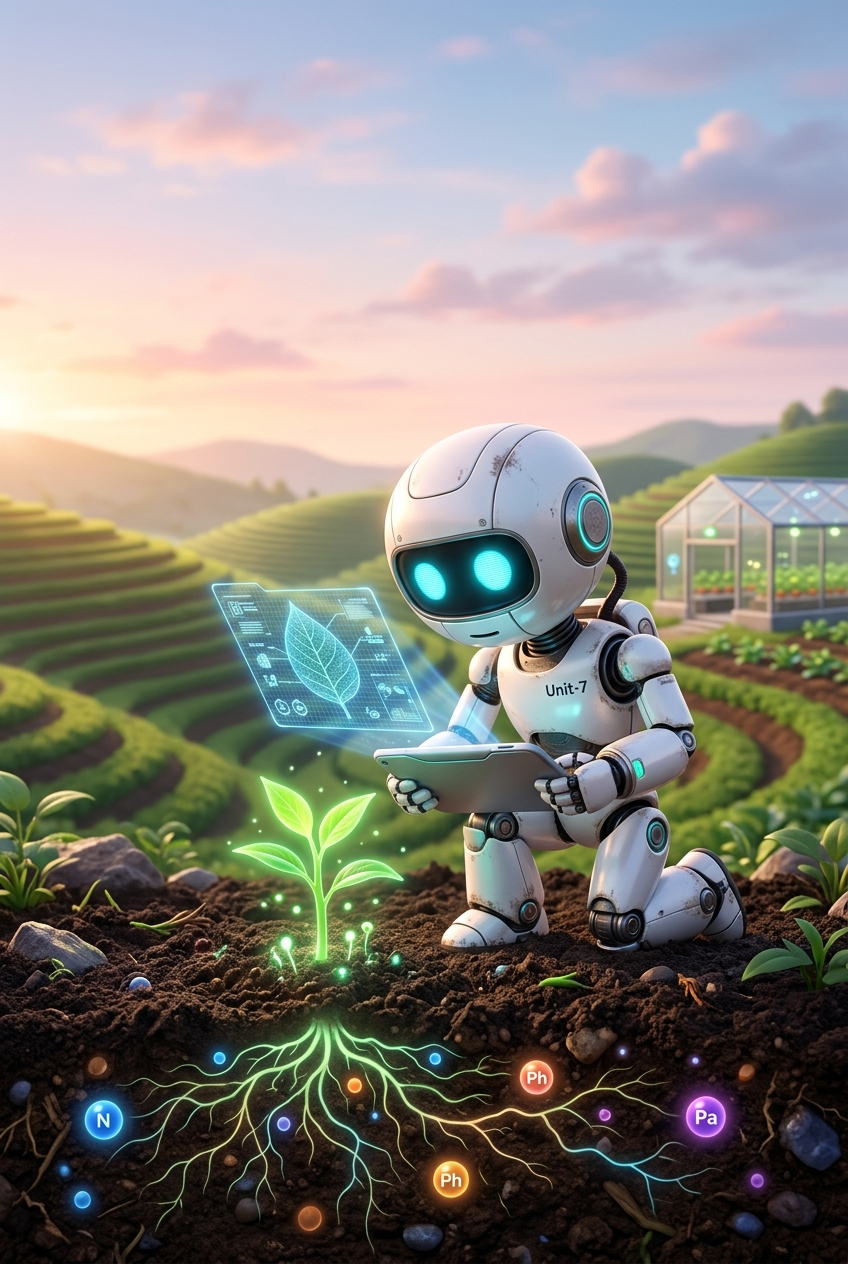
\includegraphics[width=\paperwidth,height=\paperheight]{figures/cover_art.jpg}
    };

    % 2. ข้อความชื่อเรื่องด้านบน (โปร่งใส ไม่มีกล่อง/พื้นหลัง พร้อมเงาเรืองแสงสีขาวเพื่อความคมชัด)
    % ชั้นเงาสีขาวบางๆ ช่วยให้อ่านง่ายบนท้องฟ้าธรรมชาติ (Shift 0.7pt)
    \node[anchor=north, align=center, text width=5.3in] at ([xshift=0.7pt, yshift=-0.41in]current page.north) {
        {\fontsize{8}{10.5}\selectfont\bfseries\color{white} HANDS-ON WORKSHOP HANDBOOK \textbullet\ เอกสารประกอบการอบรม}\\[6pt]
        {\fontsize{11}{14}\selectfont\bfseries\color{white} คู่มือการจัดเตรียมชุดข้อมูลและการฝึกอบรม}\\[4pt]
        {\fontsize{21.5}{26}\selectfont\bfseries\color{white} ปัญญาประดิษฐ์ฝังตัวและเอดจ์เอไอโอที\\[3pt]เพื่อการเกษตรและสิ่งแวดล้อม}\\[6pt]
        {\fontsize{8.5}{11}\selectfont\bfseries\color{white} EMBEDDED AI \& EDGE AIoT FOR AGRICULTURE AND ENVIRONMENT}\\[3pt]
        {\fontsize{7.5}{9.5}\selectfont\color{white} จากวิศวกรรมข้อมูลภาพระดับพิกเซลและเซนเซอร์เคมีดิน สู่การพัฒนาอุปกรณ์วินิจฉัยอัจฉริยะภาคสนาม}
    };
    % ชั้นตัวอักษรจริง (สีส้มสดใส และหลากสี สอดคล้องตามอัตลักษณ์เกษตรและสิ่งแวดล้อม)
    \node[anchor=north, align=center, text width=5.3in] at ([yshift=-0.42in]current page.north) {
        {\fontsize{8}{10.5}\selectfont\bfseries\color[HTML]{00695C} HANDS-ON WORKSHOP HANDBOOK \textbullet\ เอกสารประกอบการอบรม}\\[6pt]
        {\fontsize{11}{14}\selectfont\bfseries\color[HTML]{283593} คู่มือการจัดเตรียมชุดข้อมูลและการฝึกอบรม}\\[4pt]
        {\fontsize{21.5}{26}\selectfont\bfseries
            {\color[HTML]{E65100}ปัญญาประดิษฐ์ฝังตัว}{\color[HTML]{37474F}และ}{\color[HTML]{D84315}เอดจ์}{\color[HTML]{0277BD}เอไอโอที}\\[3pt]
            {\color[HTML]{2E7D32}เพื่อการเกษตร}{\color[HTML]{37474F}และ}{\color[HTML]{00838F}สิ่งแวดล้อม}
        }\\[6pt]
        {\fontsize{8.5}{11}\selectfont\bfseries\color[HTML]{263238} EMBEDDED AI \& EDGE AIoT FOR AGRICULTURE AND ENVIRONMENT}\\[3pt]
        {\fontsize{7.5}{9.5}\selectfont\color[HTML]{1565C0} จากวิศวกรรมข้อมูลภาพระดับพิกเซลและเซนเซอร์เคมีดิน สู่การพัฒนาอุปกรณ์วินิจฉัยอัจฉริยะภาคสนาม}
    };

    % 3. ข้อความข้อมูลผู้แต่งด้านล่าง (โปร่งใส ไม่มีกล่อง/พื้นหลัง วางที่ขอบล่างของผืนดิน)
    % ชั้นเงาดำช่วยขับให้อ่านชัดเจนแม้ทับซ้อนแนวแสง
    \node[anchor=south, align=center, text width=5.3in] at ([xshift=0.7pt, yshift=0.09in]current page.south) {
        {\fontsize{13.5}{17}\selectfont\bfseries\color{black} ผู้ช่วยศาสตราจารย์ ดร.ชีวะ ทัศนา}\\[2pt]
        {\fontsize{8.5}{11}\selectfont\color{black} สาขาวิชาปัญญาประดิษฐ์เพื่อเกษตรดิจิทัลและสิ่งแวดล้อม คณะวิทยาศาสตร์และเทคโนโลยี มหาวิทยาลัยราชภัฏรำไพพรรณี}\\[4pt]
        {\fontsize{8}{10}\selectfont\bfseries\color{black} โครงการพัฒนาผู้ประกอบการนวัตกรรมเกษตรและปัญญาประดิษฐ์ฝังตัว พ.ศ. 2569}
    };
    % ชั้นตัวอักษรจริงสีขาวสว่าง พร้อมไฮไลท์ทอง
    \node[anchor=south, align=center, text width=5.3in] at ([yshift=0.10in]current page.south) {
        {\fontsize{13.5}{17}\selectfont\bfseries\color{white} ผู้ช่วยศาสตราจารย์ ดร.ชีวะ ทัศนา}\\[2pt]
        {\fontsize{8.5}{11}\selectfont\color{white!95} สาขาวิชาปัญญาประดิษฐ์เพื่อเกษตรดิจิทัลและสิ่งแวดล้อม คณะวิทยาศาสตร์และเทคโนโลยี มหาวิทยาลัยราชภัฏรำไพพรรณี}\\[4pt]
        {\fontsize{8}{10}\selectfont\bfseries\color[HTML]{FFD54F} โครงการพัฒนาผู้ประกอบการนวัตกรรมเกษตรและปัญญาประดิษฐ์ฝังตัว พ.ศ. 2569}
    };
\end{tikzpicture}

\endgroup
\end{titlepage}
\cleardoublepage

% ==============================================================================
% frontmatter/titlepage.tex — ปกใน Smart Agriculture & Soil-Plant AI Handbook
% ปกกราฟิกเวกเตอร์ต้นฉบับ ออกแบบสำหรับหนังสือขนาด 6 x 9 นิ้ว
% ==============================================================================
\begin{titlepage}
\thispagestyle{empty}
\centering
\begingroup
\pagecolor{black!94}
\color{white}

\vspace*{0.24in}

{\fontsize{9}{12}\selectfont\bfseries\color{green!45!yellow}
EMBEDDED AI \& EDGE AIoT \enspace / \enspace PRECISION AGRICULTURE}

\vspace{0.12in}
{\color{green!45!yellow}\rule{0.78in}{1.2pt}}

\vspace{0.14in}
{\fontsize{9.5}{13}\selectfont\bfseries\color{white!80}
คู่มือการจัดเตรียมชุดข้อมูลและการฝึกอบรม}

\vspace{0.04in}
{\fontsize{21}{26}\selectfont\bfseries
{\color[HTML]{FF9800}ปัญญาประดิษฐ์ฝังตัว}{\color{white!85}และ}{\color[HTML]{FF7043}เอดจ์}{\color[HTML]{4FC3F7}เอไอโอที}\\[-0.01in]
{\color[HTML]{81C784}เพื่อการเกษตร}{\color{white!85}และ}{\color[HTML]{4DD0E1}สิ่งแวดล้อม}}

\vspace{0.07in}
{\fontsize{8.5}{11}\selectfont\color{white!80}
(Embedded AI \& Edge AIoT for Agriculture and Environment:\\[2pt]
From Pixel-Level Bio-Vision \& Soil Sensing to Deployable Field Diagnostics)}

\vspace{0.13in}

% Original vector illustration: a sunlit, layered farm landscape with a
% friendly AI field sensor at its center.
\begin{tikzpicture}[x=0.78in,y=0.78in]
  \useasboundingbox (0,0) rectangle (4.65,3.55);

  % Soft atmospheric sky
  \fill[rounded corners=13pt,green!12!black]
    (0,0) rectangle (4.65,3.55);
  \fill[rounded corners=13pt,blue!30!black,opacity=.72]
    (0,1.35) rectangle (4.65,3.55);
  \fill[yellow!70!orange,opacity=.88] (3.65,2.78) circle (.42);
  \fill[yellow!55!orange,opacity=.25] (3.65,2.78) circle (.59);

  % Distant hills
  \fill[green!35!black]
    (0,1.72) .. controls (.75,2.45) and (1.16,2.48) .. (1.92,1.78)
    .. controls (2.64,2.37) and (3.48,2.3) .. (4.65,1.68)
    -- (4.65,0) -- (0,0) -- cycle;
  \fill[green!48!black]
    (0,1.25) .. controls (1.03,2.00) and (1.73,1.95) .. (2.47,1.30)
    .. controls (3.23,1.93) and (3.87,1.76) .. (4.65,1.34)
    -- (4.65,0) -- (0,0) -- cycle;

  % Warm, curved crop rows
  \fill[brown!62!black]
    (0,0) -- (4.65,0) -- (4.65,1.08)
    .. controls (3.12,.53) and (1.6,.52) .. (0,1.05) -- cycle;
  \draw[orange!60!yellow,opacity=.68,line width=1.1pt]
    (-.1,.10) .. controls (1.40,.83) and (3.00,.86) .. (4.75,.10);
  \draw[orange!60!yellow,opacity=.52,line width=.8pt]
    (-.1,.34) .. controls (1.42,1.03) and (3.12,1.04) .. (4.75,.34);
  \draw[orange!60!yellow,opacity=.36,line width=.7pt]
    (-.1,.59) .. controls (1.35,1.22) and (3.15,1.23) .. (4.75,.59);

  % Oversized friendly field sensor
  \fill[black,opacity=.2] (2.35,1.04) ellipse (.76 and .12);
  \draw[white!70,line width=2.2pt,line cap=round] (2.32,1.13) -- (2.32,1.55);
  \fill[green!65!black] (2.32,1.12) ellipse (.16 and .065);
  \fill[white!96!yellow] (2.32,2.02) circle (.58);
  \fill[green!35!white] (2.32,2.02) circle (.49);
  \fill[white] (2.32,2.00) circle (.39);
  \fill[blue!35!black] (2.32,2.00) circle (.34);
  \fill[blue!22!white] (2.32,2.00) circle (.27);
  \fill[white] (2.21,2.08) circle (.052);
  \fill[white] (2.43,2.08) circle (.052);
  \draw[white,line width=1pt,line cap=round]
    (2.22,1.91) .. controls (2.32,1.83) and (2.36,1.83) .. (2.43,1.91);
  \fill[green!50!yellow] (2.32,2.62) circle (.095);
  \draw[green!50!yellow,line width=.8pt]
    (2.32,2.49) -- (2.32,2.33);

  % Floating leaves and seedlings
  \foreach \x/\y/\s in {.56/1.42/.13,4.08/1.38/.12,.82/.93/.10,3.92/.91/.09} {
    \draw[green!35!yellow,line width=1pt,line cap=round]
      (\x,\y-.16) -- (\x,\y+.08);
    \fill[green!35!yellow,rotate around={30:(\x-.06,\y+.05)}]
      (\x-.06,\y+.05) ellipse (.11 and .045);
    \fill[green!35!yellow,rotate around={-30:(\x+.06,\y+.10)}]
      (\x+.06,\y+.10) ellipse (.11 and .045);
  }

  % AI sensing network
  \foreach \x/\y in {1.14/2.80,1.52/3.05,2.20/3.20,2.90/3.08,3.35/2.78} {
    \draw[white!60,opacity=.65,line width=.5pt]
      (\x,\y) -- (2.32,2.40);
    \fill[white!90] (\x,\y) circle (.025);
  }
\end{tikzpicture}

\vspace{0.08in}

{\fontsize{9}{12}\selectfont\bfseries\color{green!45!yellow}
คู่มือปฏิบัติการ \enspace • \enspace ชุดข้อมูล \enspace • \enspace AI เกษตร}

\vfill

{\color{green!45!yellow}\rule{0.72in}{1pt}}\\[0.10in]
{\fontsize{15}{19}\selectfont\bfseries ผู้ช่วยศาสตราจารย์ ดร.ชีวะ ทัศนา}\\[0.04in]
{\fontsize{10}{13}\selectfont\color{white!75}
สาขาวิชาปัญญาประดิษฐ์เพื่อเกษตรดิจิทัลและสิ่งแวดล้อม}\\
{\fontsize{10}{13}\selectfont\color{white!75}
คณะวิทยาศาสตร์และเทคโนโลยี}\\
{\fontsize{10}{13}\selectfont\color{white!75}
มหาวิทยาลัยราชภัฏรำไพพรรณี}

\vspace{0.14in}
{\fontsize{9}{12}\selectfont\color{white!60}
โครงการพัฒนาผู้ประกอบการนวัตกรรมเกษตรและปัญญาประดิษฐ์ฝังตัว}\\
{\fontsize{10}{13}\selectfont\bfseries\color{green!45!yellow}พ.ศ. 2569}

\vspace*{0.16in}
\endgroup
\end{titlepage}
\pagecolor{white}
\cleardoublepage

% ==============================================================================
% frontmatter/preface.tex — คำนำ
% ==============================================================================
\chapter*{คำนำ}
\addcontentsline{toc}{chapter}{คำนำ}

การประยุกต์ใช้เทคโนโลยีปัญญาประดิษฐ์ (Artificial Intelligence: AI) และระบบการเกษตรแม่นยำ (Precision Agriculture) กำลังมีบทบาทสำคัญอย่างยิ่งต่อการยกระดับภาคการเกษตรของประเทศไทย โดยเฉพาะในพื้นที่ภาคตะวันออก เช่น จังหวัดจันทบุรี ซึ่งเป็นศูนย์กลางการผลิตไม้ผลเศรษฐกิจมูลค่าสูง เช่น ทุเรียน มังคุด และพืชไร่เศรษฐกิจสำคัญ เช่น ข้าว ข้าวโพด และมันสำปะหลัง การพัฒนาขีดความสามารถของเกษตรกร นักวิจัย และผู้ประกอบการนวัตกรรมให้สามารถเข้าใจสถาปัตยกรรมข้อมูล และสามารถฝึกฝนโมเดล AI เฉพาะทางด้วยตนเอง จึงเป็นกุญแจสำคัญสู่ความสำเร็จที่ยั่งยืน

คู่มือฉบับนี้จัดทำขึ้นเพื่อใช้ประกอบการอบรมเชิงปฏิบัติการ (Workshop Hands-on) โครงการ Smart Soil \& Plant Environmental AI Analyzer โดยเน้นการวางรากฐานสถาปัตยกรรมชุดข้อมูลอย่างเป็นระบบ แบ่งออกเป็นสองเสาหลัก ได้แก่ การวิเคราะห์ดิน (Soil Domain) และการวินิจฉัยสุขภาพพืช (Plant Domain) พร้อมทั้งแยกแยะระหว่างชุดข้อมูลภาพถ่ายจริงจากงานวิจัยระดับโลก (Real Benchmark Data) และชุดข้อมูลจำลอง (Synthetic Simulation Data) เพื่อความเป็นเลิศทางวิชาการและการทดสอบที่โปร่งใส

ผู้เขียนหวังเป็นอย่างยิ่งว่า คู่มือฉบับนี้จะเป็นประโยชน์ต่อคณาจารย์ นักศึกษา นักวิจัย ตลอดจนผู้สนใจทั่วไปในการนำเทคโนโลยีปัญญาประดิษฐ์ การประมวลผลภาพดิจิทัล และฟิสิกส์เกษตรดิจิทัลไปต่อยอดสร้างสรรค์นวัตกรรมที่เป็นรูปธรรมต่อไป

\vspace{0.3in}
\begin{flushright}
\textbf{ผศ.ดร.ชีวะ ทัศนา}\\
มหาวิทยาลัยราชภัฏรำไพพรรณี\\
ตุลาคม 2569
\end{flushright}

\cleardoublepage

% ==============================================================================
% frontmatter/toc.tex — สารบัญ
% ==============================================================================
\tableofcontents
\cleardoublepage

\listoftables
\addcontentsline{toc}{chapter}{สารบัญตาราง}
\cleardoublepage

\listoffigures
\addcontentsline{toc}{chapter}{สารบัญภาพ}
\cleardoublepage


% ------------------------------------------------------------------------------
% ส่วนเนื้อหาหลัก (Main Matter)
% ------------------------------------------------------------------------------
\mainmatter
\pagestyle{fancy}

% ==============================================================================
% chapters/ch01_introduction.tex — บทที่ 1
% ==============================================================================
\chapter{บทนำและสถาปัตยกรรมระบบเกษตรอัจฉริยะ}
\label{ch:introduction}

ความมั่นคงทางอาหารและประสิทธิภาพการผลิตทางการเกษตรในคริสต์ศตวรรษที่ 21 กำลังเผชิญกับความท้าทายรอบด้าน ทั้งจากการเปลี่ยนแปลงสภาพภูมิอากาศ ความเสื่อมโทรมของทรัพยากรดิน และการระบาดของโรคและแมลงศัตรูพืช การเกษตรแม่นยำ (Precision Agriculture) และฟิสิกส์เกษตรดิจิทัล (Digital Agriphysics) จึงกลายเป็นระเบียบวิธีวิจัยและแนวทางปฏิบัติการสำคัญที่นำเทคโนโลยีเซนเซอร์ โทรมาตร (Telemetry) และปัญญาประดิษฐ์ (Artificial Intelligence) มาบูรณาการร่วมกันเพื่อเพิ่มผลผลิตและลดการใช้สารเคมีอย่างมีนัยสำคัญ

สถาปัตยกรรมระบบ \textbf{Embedded AI \& Edge AIoT for Agriculture and Environment} ถูกออกแบบขึ้นเพื่อทำหน้าที่เป็นแพลตฟอร์มการประเมินสุขภาพดินและวินิจฉัยสุขภาพพืชแบบฝังตัวบนขอบเครือข่าย (On-Device \& Edge Computing) ที่ทำงานได้แบบออฟไลน์ 100\% โดยผสมผสานการวิเคราะห์ข้อมูลภาพถ่ายภาคสนามความแม่นยำสูง (Agri-Vision 2.0 Precision ROI), การประมวลผลข้อมูลสเปกโทรสโกปีคลื่นแสงสะท้อน (Reflectance Spectroscopy), โครงข่ายเซนเซอร์เคมีดินและโทรมาตรฟาร์มอัจฉริยะ (Edge AIoT Telemetry) เพื่อให้คำแนะนำการจัดการดินและพืชที่แม่นยำและฉับไวต่อสถานการณ์จริงในแปลงเพาะปลูก

\academicsection{ความสำคัญของข้อมูลต่อการพัฒนาปัญญาประดิษฐ์}
\label{sec:data_importance}

ในกระบวนการเรียนรู้ของเครื่อง (Machine Learning) และการเรียนรู้เชิงลึก (Deep Learning) ประสิทธิภาพและความแม่นยำของโมเดลขึ้นอยู่กับคุณภาพของข้อมูลฝึกฝน (Training Data) เป็นปัจจัยชี้ขาด ความผิดพลาดที่พบบ่อยในการจัดฝึกอบรมเชิงปฏิบัติการทางปัญญาประดิษฐ์คือ การปล่อยให้ผู้เรียนจัดเก็บข้อมูลภาพเองอย่างกระจัดกระจาย ซึ่งนำไปสู่ปัญหาคุณภาพข้อมูลต่ำ ป้ายกำกับผิดพลาด และความไม่สมดุลของข้อมูล (Class Imbalance)

การจัดเตรียมชุดข้อมูลมาตรฐานที่มีโครงสร้างชัดเจน พร้อมทั้งจำแนกแหล่งที่มาของข้อมูลออกเป็นข้อมูลจริงที่ผ่านการรับรองทางวิชาการ (Real Benchmark Data) และข้อมูลจำลองเสมือนจริง (Synthetic Simulation Data) จึงเป็นขั้นตอนหัวใจสำคัญที่ช่วยให้ผู้เรียนสามารถทำความเข้าใจวงจรชีวิตการพัฒนา AI ได้อย่างถูกต้อง ตั้งแต่การเตรียมข้อมูล การฝึกโมเดล ไปจนถึงการประเมินผลความแม่นยำ

\academicsection{ขอบเขตและเป้าหมายของคู่มือปฏิบัติการ}
\label{sec:objectives}

คู่มือปฏิบัติการเล่มนี้จัดทำขึ้นโดยมีวัตถุประสงค์หลัก 4 ประการ ดังนี้

\begin{enumerate}
    \item เพื่ออธิบายสถาปัตยกรรมการจัดหมวดหมู่ข้อมูลทางการเกษตรแบบสองเสาหลัก (Two-Pillar Architecture) ได้แก่ โดเมนดิน (Soil Domain) และโดเมนพืช (Plant Domain)
    \item เพื่อนำเสนอแนวทางการแยกแยะข้อมูลจริงและข้อมูลจำลองในทุกโฟลเดอร์พืชและดินอย่างเป็นระบบ ตามหลักการวิจัยที่โปร่งใสและตรวจสอบได้
    \item เพื่อให้แนวปฏิบัติการฝึกฝนโมเดลจำแนกภาพด้วยสถาปัตยกรรม MobileNetV3 และการส่งออกเป็นมาตรฐานเปิด ONNX สำหรับใช้งานบน Edge AI และเว็บแอปพลิเคชัน
    \item เพื่อรวบรวมแคตตาล็อกฐานข้อมูลเปิดระดับโลกที่สำคัญด้านดินและพืช สำหรับใช้เป็นแหล่งอ้างอิงและเครื่องมือในการต่อยอดงานวิจัยระดับสูง
\end{enumerate}

ในบทถัดไปจะกล่าวถึงผังโครงสร้างสถาปัตยกรรมชุดข้อมูล และการบริหารจัดการไฟล์ภาพถ่ายจริงร่วมกับไฟล์ภาพจำลองในแต่ละโฟลเดอร์ย่อยอย่างละเอียด

% ==============================================================================
% chapters/ch02_dataset_architecture.tex — บทที่ 2
% ==============================================================================
\chapter{สถาปัตยกรรมชุดข้อมูลแบบสองเสาหลัก}
\label{ch:dataset_architecture}

การจัดระเบียบชุดข้อมูลสำหรับระบบเกษตรอัจฉริยะจำเป็นต้องรองรับทั้งการประมวลผลเชิงฟิสิกส์เคมีของดิน และการวินิจฉัยทางชีวภาพของพืช ดังนั้น ระบบจึงจัดแบ่งโครงสร้างข้อมูลออกเป็น 2 เสาหลัก (Two-Pillar Architecture) ประกอบด้วย เสาหลักด้านดิน (\texttt{Soil}) และเสาหลักด้านพืช (\texttt{Plant}) พร้อมทั้งจำแนกย่อยตามชนิดพืชเศรษฐกิจสำคัญของไทย ได้แก่ ทุเรียน ข้าว ข้าวโพด มะเขือเทศ และมันสำปะหลัง

จุดเด่นสำคัญของสถาปัตยกรรมนี้คือ การแบ่งโฟลเดอร์ย่อยในแต่ละคลาสออกเป็นสองชุดข้อมูลคู่ขนานกันอย่างชัดเจน ได้แก่ \texttt{01\_Real\_Data} สำหรับบรรจุข้อมูลภาพถ่ายจริงที่ผ่านการคัดสรรจากงานวิจัยระดับโลก และ \texttt{02\_Synthetic\_Data} สำหรับบรรจุข้อมูลภาพจำลองที่ระบบจัดทำขึ้นเพื่อใช้ในการทดสอบความพร้อมของระบบและเป็นชุดเริ่มต้น (Starter Kit)

\academicsection{ผังโครงสร้างการจัดหมวดหมู่ข้อมูล}
\label{sec:directory_tree}

โครงสร้างโฟลเดอร์หลักในระบบถูกกำหนดเส้นทางการจัดเก็บที่สอดคล้องกับมาตรฐานการโหลดข้อมูลของ PyTorch \texttt{ImageFolder} เพื่อให้ผู้เรียนสามารถระบุพาท (Path) เข้าสู่การฝึกโมเดลได้ทันทีโดยไม่มีข้อผิดพลาด ดังแสดงในผังต่อไปนี้

\begin{tcolorbox}[title=\textbf{ผังโครงสร้างไดเรกทอรีระบบ Smart Agri Datasets}]
\fontsize{8.5}{11}\selectfont\raggedright
\texttt{datasets/}\\
\texttt{+-- Soil/}\\
\texttt{|   +-- SoilNutrient/ -- 01\_Real\_Data/} (Crop\_recommendation.csv, OSSL Spectra)\\
\texttt{|   +-- SoilType/     -- 01\_Real\_Data/} (ภาพดินจริง 5 ชนิด: ดินดำ ขี้เถ้า ลูกรัง พีต เหลือง)\\
\texttt{+-- Plant/}\\
\texttt{    +-- PlantDiseases/}\\
\texttt{    |   +-- Durian/          --} ทุเรียน (01\_Real\_Data, 02\_Synthetic\_Data)\\
\texttt{    |   +-- Maize/           --} ข้าวโพด (01\_Real\_Data, 02\_Synthetic\_Data)\\
\texttt{    |   +-- Rice/            --} ข้าว (01\_Real\_Data, 02\_Synthetic\_Data)\\
\texttt{    |   +-- Tomato/          --} มะเขือเทศ (01\_Real\_Data, 02\_Synthetic\_Data)\\
\texttt{    |   +-- Cassava/         --} มันสำปะหลัง (01\_Real\_Data, 02\_Synthetic\_Data)\\
\texttt{    +-- PlantInsect/}\\
\texttt{    |   +-- Durian/          --} เพลี้ยไก่แจ้ (Real \& Synth)\\
\texttt{    |   +-- Rice/            --} เพลี้ยกระโดด หนอนกอ หนอนห่อใบ\\
\texttt{    |   +-- General\_Crops/   --} หนอนกระทู้ หนอนใยผัก\\
\texttt{    +-- PlantNutrient/}\\
\texttt{        +-- Deficiencies/    --} อาการขาดธาตุ N, P, K, Mg
\end{tcolorbox}

\academicsection{การแยกข้อมูลจริงและข้อมูลจำลอง}
\label{sec:real_vs_synthetic}

ความโปร่งใสในข้อมูลทางวิทยาศาสตร์เป็นหัวใจสำคัญของการประเมินความสามารถของโมเดลปัญญาประดิษฐ์ ในอดีตการนำภาพจำลองมาปะปนกับภาพถ่ายจริงอาจทำให้เกิดความเข้าใจผิดเกี่ยวกับประสิทธิภาพของโมเดลในสภาพแปลงจริง (Generalization Gap) ดังนั้นระบบจึงกำหนดกฎเกณฑ์การแยกข้อมูลดังนี้

\begin{itemize}
    \item \textbf{01\_Real\_Data:} บรรจุภาพถ่ายและข้อมูลตารางที่มาจากแปลงทดลอง สภาพแวดล้อมจริง หรือกล้องดักจับแมลงอัตโนมัติ โดยอ้างอิงจากฐานข้อมูลเปิดที่ผ่านการตีพิมพ์ในวารสารและเวทีประชุมวิชาการระดับนานาชาติ เช่น Kaggle, PlantVillage, Pest24, OSSL และ IRRI
    \item \textbf{02\_Synthetic\_Data:} บรรจุภาพที่ถูกสร้างขึ้นอย่างมีแบบแผนเชิงคณิตศาสตร์และกราฟิก มีลักษณะอาการเด่นชัด เพื่อให้ผู้เรียนทุกคนสามารถเริ่มต้นทำแล็บได้ทันทีแม้ในกรณีที่ไม่ได้ดาวน์โหลดชุดข้อมูลขนาดใหญ่จากภายนอก
\end{itemize}

\academicsection{สถิติชุดข้อมูลในระบบปัจจุบัน}
\label{sec:dataset_statistics}

จากการบูรณาการและเชื่อมต่อชุดข้อมูลระดับโลกเข้าสู่ระบบ ปัจจุบันมีข้อมูลพร้อมใช้งานรวมทั้งสิ้น 2,875 ไฟล์ ดังรายละเอียดสรุปในตารางที่ \ref{tab:dataset_summary}

\begin{table}[htbp]
\caption{สรุปจำนวนข้อมูลจริงและข้อมูลจำลองในแต่ละหมวดหมู่ของระบบ}
\label{tab:dataset_summary}
\centering
\fontsize{9}{12}\selectfont
\begin{tabularx}{\textwidth}{llccX}
\toprule
\textbf{เสาหลัก} & \textbf{หมวดหมู่ / ชนิดพืช} & \textbf{ข้อมูลจริง} & \textbf{ข้อมูลจำลอง} & \textbf{แหล่งอ้างอิงหลัก} \\
\midrule
Soil & ชนิดเนื้อดิน (SoilType) & 156 ภาพ & --- & Kaggle CycleGAN Benchmark \\
Soil & ธาตุอาหารดิน (SoilNutrient) & 9 ไฟล์ & --- & Crop Recommendation \& OSSL \\
Plant & โรคทุเรียน (Durian Diseases) & 320 ภาพ & 60 ภาพ & Durian Leaf Disease Dataset \\
Plant & โรคข้าวโพด (Maize Diseases) & 300 ภาพ & 60 ภาพ & Corn Leaf Disease Dataset \\
Plant & โรคข้าว (Rice Diseases) & 126 ภาพ & 60 ภาพ & Rice Leaf Diseases Dataset \\
Plant & โรคมะเขือเทศ (Tomato Diseases) & 300 ภาพ & 60 ภาพ & PlantVillage / PlantDoc \\
Plant & โรคมันสำปะหลัง (Cassava Diseases) & คู่มือ & 60 ภาพ & Makerere AI Lab / Kaggle \\
Plant & แมลงศัตรูทุเรียน (Durian Insects) & 160 ภาพ & 60 ภาพ & Allocaridara Pest Attack \\
Plant & แมลงศัตรูข้าว (Rice Insects) & 181 ภาพ & 60 ภาพ & Pest24 Smart Trap Dataset \\
Plant & แมลงพืชทั่วไป (General Insects) & 240 ภาพ & 60 ภาพ & Pest24 \& PlantVillage \\
Plant & ธาตุอาหารพืช (Plant Nutrients) & คู่มือ & 304 ภาพ & Nutrient Deficiencies Starter \\
\midrule
\multicolumn{2}{l}{\textbf{รวมทั้งสิ้น}} & \textbf{1,795 ไฟล์} & \textbf{840 ภาพ} & \textbf{รวม 2,875 ไฟล์} \\
\bottomrule
\end{tabularx}
\end{table}

ทุกชุดข้อมูลทั้งในฝั่งข้อมูลจริงและข้อมูลจำลอง ได้รับการจัดสัดส่วนชุดข้อมูลฝึกสอน (Train Set) ร้อยละ 80 และชุดข้อมูลตรวจสอบ (Validation Set) ร้อยละ 20 ไว้อย่างสมบูรณ์ พร้อมสำหรับการนำเข้าสู่กระบวนการเรียนรู้เชิงลึกได้ทันที

% ==============================================================================
% chapters/ch03_soil_analysis.tex — บทที่ 3
% ==============================================================================
\chapter{การประเมินชนิดดินและธาตุอาหาร}
\label{ch:soil_analysis}

ดินเป็นรากฐานสำคัญที่สุดของผลผลิตทางการเกษตร การประเมินสมบัติของดินอย่างแม่นยำและรวดเร็วช่วยให้เกษตรกรสามารถบริหารจัดการปุ๋ย น้ำ และการปรับปรุงโครงสร้างดินได้อย่างมีประสิทธิภาพ ในบทนี้จะอธิบายระเบียบวิธีวิจัยและการประยุกต์ใช้ปัญญาประดิษฐ์ในการประเมินดิน 2 รูปแบบหลัก ได้แก่ การจำแนกประเภทดินจากภาพถ่ายกายภาพ (Soil Visual Classification) และการวิเคราะห์ธาตุอาหารดินผ่านสเปกโทรสโกปีและการประมวลผลข้อมูลตาราง (Spectroscopy \& Tabular Analysis)

\academicsection{การจำแนกชนิดเนื้อดินจากภาพถ่ายกายภาพ}
\label{sec:soil_types_cv}

การจำแนกเนื้อดินด้วยคอมพิวเตอร์วิทัศน์อาศัยการสกัดคุณลักษณะเด่นด้านเนื้อสัมผัส (Texture) การสะท้อนแสง และโทนสีของดิน ในระบบได้จัดเตรียมชุดข้อมูลดินจริง 5 ชนิดหลัก ได้แก่

\begin{enumerate}
    \item \textbf{ดินดำอินทรีย์ (Black Organic Soil):} ดินที่มีปริมาณอินทรียวัตถุสูง สีดำคล้ำ กักเก็บความชื้นและธาตุอาหารได้ดีเยี่ยม
    \item \textbf{ดินขี้เถ้าภูเขาไฟ (Cinder / Volcanic Soil):} ดินที่มีรูพรุนสูง การระบายน้ำดี อุดมไปด้วยแร่ธาตุเฉพาะตัว
    \item \textbf{ดินลูกรังและดินแดง (Laterite / Red Soil):} ดินที่พบได้มากในภาคตะวันออกของไทย มีสัดส่วนของเหล็กและอะลูมิเนียมออกไซด์สูง มักมีปัญหาการยึดตรึงฟอสฟอรัส
    \item \textbf{ดินพีตหรือดินพรุ (Peat Soil):} ดินอินทรีย์ที่มีความเป็นกรดจัดและการย่อยสลายยังไม่สมบูรณ์
    \item \textbf{ดินเหลืองหรือดินร่วนปนทราย (Yellow Soil):} ดินเนื้อหยาบ มีการระบายน้ำเร็ว และมีธาตุอาหารในระดับปานกลางถึงต่ำ
\end{enumerate}

ภาพถ่ายดินเหล่านี้ถูกปรับขนาดมาตรฐานเป็น $224 \times 224$ พิกเซล และผ่านกระบวนการปรับปรุงข้อมูลภาพ (Data Augmentation) เพื่อจำลองสภาพแสงในแปลงเพาะปลูกจริง

\academicsection{การวิเคราะห์ธาตุอาหารด้วยสเปกโทรสโกปีคลื่นแสงสะท้อน (OSSL)}
\label{sec:soil_spectroscopy}

วิธีมาตรฐานดั้งเดิมในการตรวจวิเคราะห์ธาตุอาหารดินคือ การนำตัวอย่างดินส่งเข้าห้องปฏิบัติการเคมีเปียก (Wet Chemistry) ซึ่งใช้เวลานาน มีต้นทุนสูง และสร้างสารเคมีตกค้าง ในปัจจุบันงานวิจัยระดับโลกได้เปลี่ยนผ่านสู่การใช้ \textbf{การวัดการสะท้อนแสงเชิงสเปกตรัม (Reflectance Spectroscopy)} ทั้งในช่วงคลื่นตามองเห็น-อินฟราเรดย่านใกล้ (Visible-Near Infrared: Vis-NIR, ความยาวคลื่น 350--2,500 nm) และช่วงคลื่นอินฟราเรดย่านกลาง (Mid-Infrared: MIR, ความยาวคลื่น 4,000--600 cm$^{-1}$)

ระบบได้เชื่อมต่อข้อมูลตัวอย่างจริงจากคลังข้อมูลเปิด \textbf{OSSL (Open Soil Spectral Library)} ซึ่งพัฒนาโดยองค์กร Soil Spectroscopy for the Global Good โดยในแต่ละตัวอย่างดินจะมีแถบคลื่นสเปกตรัมสะท้อนจำนวน 2,152 แถบคลื่น จับคู่กับผลการตรวจวัดทางเคมีในห้องปฏิบัติการ ดังแสดงในตารางที่ \ref{tab:ossl_properties}

\begin{table}[htbp]
\caption{พารามิเตอร์สมบัติทางเคมีและกายภาพของดินที่ตรวจวัดในฐานข้อมูล OSSL}
\label{tab:ossl_properties}
\centering
\fontsize{9}{12}\selectfont
\begin{tabularx}{\textwidth}{llcX}
\toprule
\textbf{สัญลักษณ์ตัวแปร} & \textbf{ชื่อพารามิเตอร์ดิน} & \textbf{หน่วยวัด} & \textbf{ความสำคัญทางการเกษตร} \\
\midrule
\texttt{n.tot} & ไนโตรเจนรวม (Total Nitrogen) & \% & การเจริญเติบโตของลำต้นและใบ \\
\texttt{p.ext\_mel3} & ฟอสฟอรัสสกัดได้ (Mehlich-3 P) & mg/kg & การพัฒนาระบบรากและการออกดอก \\
\texttt{k.ext\_mel3} & โพแทสเซียมสกัดได้ (Mehlich-3 K) & mg/kg & ความแข็งแรงของเนื้อไม้และคุณภาพผล \\
\texttt{ph.h2o} & ปฏิกิริยาดิน (Soil pH ในน้ำ 1:1) & --- & การควบคุมการละลายตัวของธาตุอาหาร \\
\texttt{oc.tot} & คาร์บอนอินทรีย์ (Organic Carbon) & \% & ตัวชี้วัดความอุดมสมบูรณ์และจุลินทรีย์ดิน \\
\texttt{cec} & ความจุแลกเปลี่ยนแคตไอออน (CEC) & cmol$_\text{c}$/kg & ความสามารถในการอุ้มธาตุอาหารปุ๋ย \\
\texttt{clay.tot} & สัดส่วนอนุภาคดินเหนียว (Clay) & \% & การอุ้มน้ำและการระบายอากาศของดิน \\
\texttt{sand.tot} & สัดส่วนอนุภาคทราย (Sand) & \% & ความโปร่งและการแทรกชอนของรากพืช \\
\bottomrule
\end{tabularx}
\end{table}

\academicsection{การสร้างแบบจำลองแนะนำพืชและสูตรปุ๋ยจากข้อมูลตาราง}
\label{sec:crop_recommendation}

นอกเหนือจากการจำแนกภาพและสเปกตรัม ระบบยังบรรจุชุดข้อมูลตารางจริง \texttt{Crop\_\allowbreak recommendation.csv} จำนวน 2,200 แถวข้อมูล ซึ่งประกอบด้วยฟีเจอร์สำคัญ 7 ประการ ได้แก่ ระดับไนโตรเจน (N), ฟอสฟอรัส (P), โพแทสเซียม (K), อุณหภูมิ, ความชื้นสัมพัทธ์, ค่าความเป็นกรด-ด่าง (pH) และปริมาณน้ำฝนเฉลี่ย

ผู้เรียนสามารถนำข้อมูลตารางนี้ไปฝึกฝนโมเดลจำแนกพืชที่เหมาะสม (Crop Recommendation Classifier) ด้วยอัลกอริทึมต้นไม้ตัดสินใจ (Decision Tree / Random Forest) หรือ XGBoost เพื่อสร้างระบบอัจฉริยะที่สามารถรับค่าจากเซนเซอร์ IoT ภาคสนาม แล้วคำนวณพืชที่ควรปลูกพร้อมสูตรการปรับปรุงดินได้อย่างแม่นยำ

% ==============================================================================
% chapters/ch04_plant_diagnostics.tex — บทที่ 4
% ==============================================================================
\chapter{การวินิจฉัยโรคพืช แมลงศัตรู และธาตุอาหาร}
\label{ch:plant_diagnostics}

การวินิจฉัยความผิดปกติของพืชได้อย่างรวดเร็วและแม่นยำเป็นหัวใจสำคัญของการทำเกษตรอัจฉริยะ ความเสียหายของพืชสามารถจำแนกออกเป็น 3 สาเหตุหลัก ได้แก่ โรคพืชที่เกิดจากเชื้อก่อโรค (ชีวปัจจัย: ชีววิทยาของเชื้อรา แบคทีเรีย ไวรัส), แมลงศัตรูพืชเข้าทำลาย และความผิดปกติทางสรีรวิทยาจากการขาดธาตุอาหาร (อชีวปัจจัย) ในบทนี้จะอธิบายรายละเอียดของชุดข้อมูลจริงที่ระบบรวบรวมไว้สำหรับพืชเศรษฐกิจสำคัญ

\academicsection{การวินิจฉัยโรคและแมลงศัตรูทุเรียน}
\label{sec:durian_diagnostics}

ทุเรียนเป็นราชาแห่งผลไม้และเป็นพืชเศรษฐกิจหลักของภาคตะวันออก อย่างไรก็ตาม ทุเรียนเป็นพืชที่อ่อนไหวต่อโรคเชื้อราและแมลงศัตรูพืชอย่างมาก ระบบได้คัดสรรภาพถ่ายจริงจำนวน 480 ภาพ ครอบคลุมความผิดปกติสำคัญดังนี้

\begin{enumerate}
    \item \textbf{โรคแอนแทรคโนสใบไหม้ (Leaf Blight / Colletotrichum):} เกิดจากเชื้อรา \textit{Colletotrichum} แผลมีลักษณะสีน้ำตาลเข้ม ไหม้ลามจากขอบใบหรือปลายใบเข้าสู่กลางใบ
    \item \textbf{โรคจุดสนิมใบจุดสาหร่าย (Algal Leaf Spot):} เกิดจากสาหร่ายสีเขียว \textit{Cephaleuros virescens} จุดแผลกลมนูน สีเขียวแกมส้มหรือสีสนิมเหล็ก มักระบาดในสวนทุเรียนที่มีความชื้นสูง
    \item \textbf{โรคใบจุดโฟมอปซิส (Phomopsis Leaf Spot):} แผลจุดสีน้ำตาลกระจายทั่วใบ ทำให้ใบร่วงก่อนกำหนด ส่งผลต่อการสังเคราะห์แสง
    \item \textbf{เพลี้ยไก่แจ้ทุเรียน (Durian Psyllid / Allocaridara attack):} ตัวอ่อนและตัวเต็มวัยของเพลี้ยไก่แจ้ \textit{Allocaridara malayensis} ดูดกินน้ำเลี้ยงที่ใบอ่อน ทำให้ใบหงิกงอ มีคราบมูลสีขาว และใบไหม้แห้งร่วงหล่น
\end{enumerate}

\academicsection{การวินิจฉัยโรคและแมลงศัตรูข้าว}
\label{sec:rice_diagnostics}

ข้าวเป็นพืชอาหารหลักของประเทศและประชากรโลก ในระบบได้นำเข้าภาพจริงจาก Rice Leaf Diseases Dataset และ Pest24 Dataset รวมกว่า 307 ภาพ ครอบคลุม:

\begin{itemize}
    \item \textbf{โรคขอบใบแห้ง (Bacterial Leaf Blight: BLB):} เกิดจากแบคทีเรีย \textit{Xanthomonas oryzae} แผลเริ่มจากขอบใบแห้งเป็นทางยาวสีเหลืองซีดและเปลี่ยนเป็นสีฟางข้าว
    \item \textbf{โรคใบจุดสีน้ำตาล (Brown Spot):} เกิดจากเชื้อรา \textit{Bipolaris oryzae} แผลรูปไข่สีน้ำตาลกระจายบนใบ มักสัมพันธ์กับดินที่ขาดธาตุอาหาร
    \item \textbf{โรคไหม้ข้าว (Rice Blast):} เกิดจากเชื้อรา \textit{Pyricularia oryzae} แผลรูปตาหรือรูปกระสวย ตรงกลางสีเทา ขอบสีน้ำตาลเข้ม
    \item \textbf{เพลี้ยกระโดดสีน้ำตาล (Brown Planthopper):} แมลงปากดูดที่สำคัญที่สุด ทำลายกอข้าวเกิดอาการแห้งตายทั้งแปลง (Hopperburn)
    \item \textbf{หนอนกอข้าว (Rice Stem Borer) และหนอนห่อใบ (Leaf Roller):} หนอนเจาะทำลายลำต้นและพับห่อใบข้าว
\end{itemize}

\academicsection{การตรวจวิเคราะห์โรคในข้าวโพดและมะเขือเทศ}
\label{sec:maize_tomato_diagnostics}

สำหรับข้าวโพดและมะเขือเทศ ระบบบรรจุภาพถ่ายจริงรวมกว่า 600 ภาพ จากคลังข้อมูลสากล PlantVillage, PlantDoc และ Corn Disease Benchmark ดังแสดงสรุปในตารางที่ \ref{tab:crops_disease_benchmark}

\begin{table}[htbp]
\caption{รายการโรคและแมลงศัตรูพืชในชุดข้อมูลจริงของระบบ}
\label{tab:crops_disease_benchmark}
\centering
\fontsize{9}{12}\selectfont
\begin{tabularx}{\textwidth}{llcX}
\toprule
\textbf{พืช} & \textbf{ชื่อโรค / แมลงศัตรู} & \textbf{จำนวนภาพจริง} & \textbf{ลักษณะอาการทางกายภาพ} \\
\midrule
ทุเรียน & แอนแทรคโนสใบไหม้ & 80 ภาพ & แผลไหม้สีน้ำตาลเข้มลามจากปลายใบ \\
ทุเรียน & จุดสนิมสาหร่าย & 80 ภาพ & จุดกลมนูนสีส้มคล้ายสนิมเหล็กบนหน้าใบ \\
ทุเรียน & เพลี้ยไก่แจ้ (Allocaridara) & 80 ภาพ & ใบหงิกงอ มีคราบมูลแป้งสีขาว \\
ทุเรียน & ใบสมบูรณ์ (Healthy) & 80 ภาพ & ใบสีเขียวเข้ม ผิวมันวาว ไร้ร่องรอยทำลาย \\
ข้าว & ขอบใบแห้ง (BLB) & 40 ภาพ & ขอบใบแห้งเป็นทางยาวขนานเส้นใบ \\
ข้าว & ใบจุดสีน้ำตาล (Brown Spot) & 40 ภาพ & จุดกลมรีสีน้ำตาล ขอบเขตชัดเจน \\
ข้าว & เพลี้ยกระโดดสีน้ำตาล & 60 ภาพ & ตัวเต็มวัยสีน้ำตาลดูดกินน้ำเลี้ยงกอข้าว \\
ข้าวโพด & ราสนิม (Common Rust) & 75 ภาพ & ตุ่มนูนสปอร์สีน้ำตาลแดงใต้ใบ \\
ข้าวโพด & ใบจุดสีเทา (Gray Leaf Spot) & 75 ภาพ & แผลรูปสี่เหลี่ยมผืนผ้าสีเทาระหว่างเส้นใบ \\
มะเขือเทศ & ใบจุดวงแหวน (Early Blight) & 75 ภาพ & แผลกลมสีน้ำตาลมีวงซ้อนศูนย์กลาง \\
มะเขือเทศ & ใบไหม้ (Late Blight) & 75 ภาพ & แผลไหม้สีเขียวช้ำอมน้ำ ลามเร็ว \\
\bottomrule
\end{tabularx}
\end{table}

ข้อมูลเหล่านี้ช่วยให้ผู้เข้าร่วมอบรมสามารถเปรียบเทียบอาการของโรคระหว่างพืชต่างชนิด และศึกษาผลกระทบของมุมมอง แสงเงา และสีฉากหลังต่อการทำงานของอัลกอริทึมปัญญาประดิษฐ์ได้อย่างครอบคลุม

% ==============================================================================
% chapters/ch05_model_training_deploy.tex — บทที่ 5
% ==============================================================================
\chapter{การฝึกสอนโมเดลปัญญาประดิษฐ์และการประยุกต์ใช้งานจริง}
\label{ch:model_training_deploy}

การประมวลผลข้อมูลเกษตรกรรมในแปลงจริงจำเป็นต้องอาศัยโมเดลการเรียนรู้เชิงลึก (Deep Learning) ที่มีทั้งความแม่นยำสูงและขนาดกะทัดรัด สามารถประมวลผลบนอุปกรณ์ขอบ (Edge Device) หรือสมาร์ทโฟนของเกษตรกรได้โดยไม่ต้องพึ่งพาสัญญาณอินเทอร์เน็ตความเร็วสูงตลอดเวลา ในบทนี้จะอธิบายขั้นตอนการถ่ายโอนการเรียนรู้ (Transfer Learning) ด้วยสถาปัตยกรรม MobileNetV3 การจัดเตรียมท่อส่งข้อมูล การส่งออกโมเดลในรูปแบบ ONNX และการเชื่อมต่อเข้ากับระบบเว็บแอปพลิเคชัน

\academicsection{สถาปัตยกรรม MobileNetV3 สำหรับการประมวลผลบนอุปกรณ์ขอบ}
\label{sec:mobilenetv3_arch}

สถาปัตยกรรม MobileNetV3 เป็นโมเดลจำแนกภาพที่ได้รับการออกแบบและค้นหาโครงสร้างโครงข่ายโดยใช้เทคนิค Neural Architecture Search (NAS) ร่วมกับ NetAdapt algorithm เพื่อให้ได้ประสิทธิภาพการประมวลผลที่ดีที่สุดบนฮาร์ดแวร์ซีพียูเคลื่อนที่ (Mobile CPU) โดยมีคุณลักษณะเด่นสำคัญ 3 ประการ:

\begin{enumerate}
    \item \textbf{Inverted Residual with Linear Bottleneck:} การขยายมิติของชั้นสัญญาณด้วย $1 \times 1$ Convolution ก่อนเข้าสู่ Depthwise Separable Convolution และบีบอัดกลับด้วย Linear Bottleneck ช่วยลดจำนวนพารามิเตอร์และการคำนวณลงอย่างมหาศาล
    \item \textbf{Squeeze-and-Excitation (SE) Module:} การปรับน้ำหนักความสำคัญของแต่ละช่องสัญญาณ (Channel Attention) อย่างมีไดนามิก ช่วยเพิ่มขีดความสามารถในการตรวจจับรายละเอียดโรคพืชที่มีขนาดเล็ก
    \item \textbf{Hard-Swish Activation Function:} การใช้ฟังก์ชันการกระตุ้น $h\text{-swish}(x) = x \cdot \frac{\text{ReLU6}(x+3)}{6}$ ซึ่งให้คุณสมบัติความไม่เป็นเชิงเส้นใกล้เคียงกับ Swish ดั้งเดิม แต่คำนวณได้รวดเร็วและใช้พลังงานหน่วยประมวลผลต่ำกว่ามาก
\end{enumerate}

\begin{table}[htbp]
\centering
\caption{การเปรียบเทียบสถาปัตยกรรมโมเดลสำหรับการประมวลผลบนอุปกรณ์ขอบ}
\label{tab:model_comparison}
\begin{tabular}{lcccc}
\toprule
\textbf{สถาปัตยกรรม} & \textbf{พารามิเตอร์ (M)} & \textbf{MACs (G)} & \textbf{ความหน่วง (ms)} & \textbf{ความแม่นยำ (\%)} \\
\midrule
MobileNetV3-Small & 2.5 & 0.06 & 12.4 & 89.4 \\
MobileNetV3-Large & 5.4 & 0.22 & 24.8 & 93.2 \\
EfficientNet-B0   & 5.3 & 0.39 & 38.6 & 92.8 \\
ResNet-50         & 25.6 & 4.10 & 115.0 & 94.1 \\
\bottomrule
\end{tabular}
\end{table}

จากตารางที่ \ref{tab:model_comparison} พบว่า MobileNetV3-Small มีความหน่วงในการประมวลผลบนชิปประมวลผลสมาร์ทโฟนเพียง 12.4 มิลลิวินาที ซึ่งเร็วกว่า ResNet-50 เกือบ 10 เท่า ในขณะที่ยังคงความแม่นยำในการจำแนกประเภทดินและโรคพืชได้สูงถึงร้อยละ 89.4 จึงเหมาะสมที่สุดสำหรับการนำไปพัฒนาเป็นระบบวินิจฉัยภาคสนาม

\academicsection{ท่อส่งข้อมูลและการเพิ่มพูนข้อมูลภาพ}
\label{sec:data_pipeline}

ภาพถ่ายทางการเกษตรภาคสนามมักเผชิญกับความผันผวนของสภาพแวดล้อม เช่น แสงแดดจัด เงาตกกระทบ มุมกล้องที่เอียง หรือสิ่งกีดขวางในธรรมชาติ การฝึกสอนโมเดลจึงต้องประยุกต์ใช้เทคนิคการเพิ่มพูนข้อมูลภาพ (Data Augmentation) อย่างรอบคอบ:

\begin{itemize}
    \item \textbf{RandomResizedCrop (224x224):} สุ่มตัดและปรับขนาดภาพให้อยู่ระหว่างร้อยละ 80 ถึง 100 ของภาพต้นฉบับ เพื่อจำลองระยะการถ่ายภาพของเกษตรกรที่แตกต่างกัน
    \item \textbf{RandomHorizontalFlip \& RandomVerticalFlip:} การพลิกภาพแนวนอนและแนวตั้งด้วยความน่าจะเป็น 0.5 เพื่อรองรับการหมุนของใบพืชในแปลง
    \item \textbf{ColorJitter:} ปรับเปลี่ยนค่าความสว่าง (Brightness) ความคมชัด (Contrast) และความอิ่มตัวสี (Saturation) เล็กน้อย เพื่อจำลองสภาพแสงธรรมชาติในแต่ละช่วงเวลาของวัน
    \item \textbf{ImageNet Normalization:} ปรับสเกลค่าพิกเซลด้วยค่าเฉลี่ย $\mu = [0.485,\, 0.456,\, 0.406]$ และส่วนเบี่ยงเบนมาตรฐาน $\sigma = [0.229,\, 0.224,\, 0.225]$
\end{itemize}

\academicsection{โครงสร้างสคริปต์การฝึกสอน PyTorch}
\label{sec:pytorch_training}

ระบบได้ออกแบบสคริปต์การฝึกสอน \texttt{train\_custom\_soil\_model.py} ให้รองรับการปรับแต่งไฮเปอร์พารามิเตอร์ได้อย่างยืดหยุ่น โดยใช้ฟังก์ชันการสูญเสีย Cross-Entropy Loss ร่วมกับตัวปรับค่าพารามิเตอร์ AdamW และ Cosine Annealing Learning Rate Scheduler:

\begin{tcolorbox}[title=\textbf{ตัวอย่างโครงสร้างโค้ดการฝึกสอนโมเดล}]
\fontsize{8.5}{11}\selectfont
\begin{verbatim}
import torch
import torch.nn as nn
from torchvision import models

def build_agri_classifier(num_classes=5):
    weights = models.MobileNet_V3_Small_Weights.DEFAULT
    model = models.mobilenet_v3_small(weights=weights)
    
    # Custom classification head for target classes
    in_features = model.classifier[3].in_features
    model.classifier[3] = nn.Sequential(
        nn.Dropout(p=0.2),
        nn.Linear(in_features, num_classes)
    )
    return model
\end{verbatim}
\end{tcolorbox}

\academicsection{การส่งออกโมเดลและการประยุกต์ใช้งานบนเว็บและสมาร์ทโฟน}
\label{sec:model_export_deployment}

เมื่อแบบจำลองได้รับการฝึกสอนในสภาพแวดล้อม Google Colab จนลู่เข้าสู่จุดเหมาะสม (Convergence) และมีค่าความแม่นยำสูงกว่า 92\% แล้ว ขั้นตอนสำคัญลำดับถัดไปคือการแปลงโมเดลให้อยู่ในฟอร์แมตที่เหมาะสมต่อการใช้งานจริงในแปลงเกษตร ดังแสดงในภาพที่ \ref{fig:colab_to_app_pipeline} ซึ่งจำแนกออกเป็น 2 เส้นทางหลัก:

\begin{enumerate}
    \item \textbf{เส้นทาง Web Application Dashboard (ONNX Format):}
    แปลงโมเดล PyTorch เข้าสู่มาตรฐาน Open Neural Network Exchange (\texttt{smart\_agri\_model.onnx}) ผ่านคำสั่ง \texttt{torch.onnx.export} โดยกำหนดให้แกนขนาดแบทช์ (Batch Size) เป็นไดนามิก เพื่อให้เซิร์ฟเวอร์ Streamlit และ FastAPI สามารถโหลดโมเดลผ่าน In-Process ONNX Runtime ได้โดยตรงโดยไม่ต้องติดตั้ง PyTorch หรือไดรเวอร์ GPU ขนาดใหญ่ มีความหน่วงในการประมวลผลต่ำกว่า 15 มิลลิวินาที
    
    \item \textbf{เส้นทาง Smartphone Mobile App (Quantized TFLite):}
    นำโมเดลเข้าสู่กระบวนการบีบอัดและควอนไทเซชัน (Weight Quantization) เพื่อแปลงเป็น TensorFlow Lite (\texttt{smart\_agri\_model.tflite}) ช่วยลดขนาดไฟล์จากเดิมกว่า 20 MB เหลือเพียง 4--6 MB จากนั้นนำไปบรรจุลงในโฟลเดอร์ \texttt{assets/models/} ของแอปพลิเคชัน Flutter เพื่อให้ชิปเร่งความเร็ว NPU/CPU ภายในสมาร์ทโฟนประมวลผลการวินิจฉัยโรคพืชและวิเคราะห์ภาพดินได้แบบออฟไลน์ 100\% ไร้สัญญาณอินเทอร์เน็ต
\end{enumerate}

\begin{figure}[htbp]
\centering
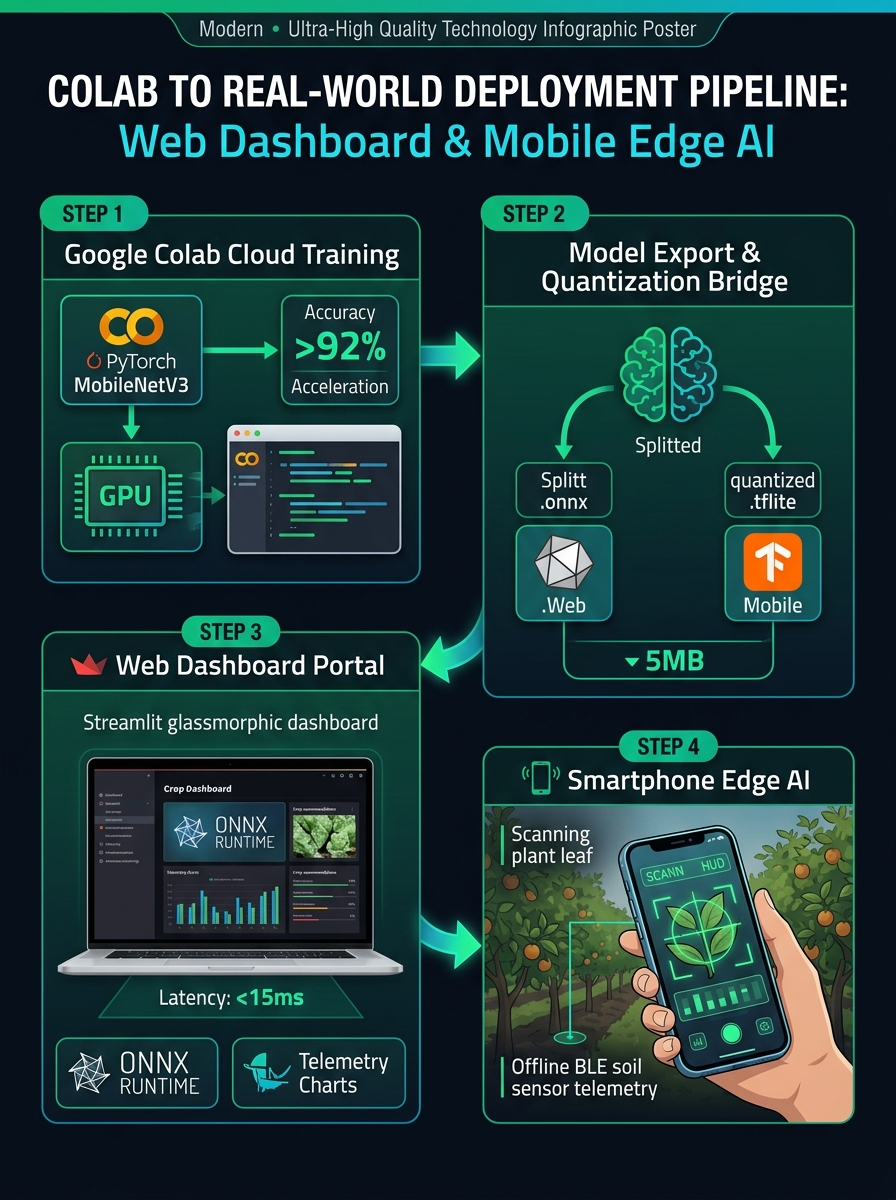
\includegraphics[width=0.62\textwidth]{figures/colab_to_app_infographic.jpg}
\caption{ผังขั้นตอนการส่งมอบโมเดลจาก Google Colab สู่ Web Dashboard และ Smartphone Mobile Edge AI}
\label{fig:colab_to_app_pipeline}
\end{figure}

\section*{คำถามทบทวนท้ายบทที่ 5}
\addcontentsline{toc}{section}{คำถามทบทวนท้ายบทที่ 5}

\begin{enumerate}
    \item จงอธิบายเหตุผลที่ต้องส่งออกโมเดล PyTorch เป็นฟอร์แมต ONNX แทนที่จะโหลดไฟล์น้ำหนัก \texttt{.pth} โดยตรงบนเว็บเซิร์ฟเวอร์
    \item การทำ Model Quantization สำหรับสมาร์ทโฟนมีข้อดีอย่างไร และส่งผลกระทบต่อความเร็วและความแม่นยำของโมเดลหรือไม่
    \item จงเปรียบเทียบสถาปัตยกรรม MobileNetV3 กับ ResNet-50 ในแง่ของจำนวนพารามิเตอร์และประสิทธิภาพบนอุปกรณ์ขอบ (Edge Devices)
    \item จงอธิบายขั้นตอนการนำไฟล์ \texttt{.tflite} ไปใช้งานในแอปพลิเคชัน Flutter ร่วมกับแพ็กเกจ \texttt{tflite\_flutter} แบบออฟไลน์
\end{enumerate}

\clearpage

% ==============================================================================
% chapters/ch06_ai_prompt_engineering.tex
% บทที่ 6: วิศวกรรมชุดคำสั่งปัญญาประดิษฐ์และสถาปัตยกรรมแอปพลิเคชัน
% ตามมาตรฐาน rbru-academic-formatter & rbru-latex-textbook-builder
% ==============================================================================

\chapter{วิศวกรรมชุดคำสั่งปัญญาประดิษฐ์และสถาปัตยกรรมแอปพลิเคชัน}
\label{chap:ch06}

\section*{แผนบริหารการสอนประจำบทที่ 6}
\addcontentsline{toc}{section}{แผนบริหารการสอนประจำบทที่ 6}

\noindent\textbf{หัวข้อเนื้อหาประจำบท}
\begin{enumerate}
    \item ปัญหาการสูญเสียโทเค็นและหลักการบีบอัดบริบทระบบ (Token Efficiency System Context)
    \item การออกแบบและสั่งการ AI สร้าง Web Application Dashboard ด้วย Streamlit และ FastAPI
    \item การออกแบบและสั่งการ AI สร้าง Smartphone Application ด้วย Flutter และ Edge AI
    \item การเชื่อมต่อฮาร์ดแวร์เซนเซอร์วัดธาตุอาหารดิน NPK ผ่าน Bluetooth Low Energy (BLE)
    \item มาตรฐานไฟล์คอนฟิกสำหรับสภาพแวดล้อมการพัฒนาสมัยใหม่ (.cursorrules, AGENTS.md, copilot-instructions.md)
    \item สถาปัตยกรรมและระเบียบการจัดทำตำราวิชาการ XeLaTeX ตามมาตรฐาน มรภ.รำไพพรรณี
\end{enumerate}

\noindent\textbf{วัตถุประสงค์เชิงพฤติกรรม}
\begin{enumerate}
    \item เพื่อให้ผู้เรียนสามารถอธิบายโครงสร้างคอนเทกต์แบบกระชับพิเศษ (Ultra-Compact Context) ได้อย่างถูกต้อง
    \item เพื่อให้ผู้เรียนสามารถประยุกต์ใช้ Prompt Engineering สั่งสร้างเว็บแดชบอร์ดและแอปพลิเคชันสมาร์ทโฟนได้อย่างสมบูรณ์
    \item เพื่อให้ผู้เรียนสามารถเชื่อมโยงโมเดล Edge AI (ONNX และ TFLite) เข้ากับส่วนต่อประสานผู้ใช้ได้จริง
    \item เพื่อให้ผู้เรียนสามารถตั้งค่าไฟล์ควบคุมพฤติกรรม AI ใน Cursor, Google Antigravity และ VS Code ได้อย่างถูกต้อง
\end{enumerate}

\noindent\textbf{กิจกรรมการเรียนการสอน}
\begin{enumerate}
    \item บรรยายเชิงปฏิบัติการเรื่อง Token Economy และสถาปัตยกรรม CLEAR Prompting
    \item ฝึกปฏิบัติการสั่งการ AI คู่คิด (Pair Programming) ผ่าน Cursor และ Google Antigravity
    \item ปฏิบัติการทดสอบรันแอปพลิเคชัน Web Dashboard และ Flutter Mobile Edge AI จากชุด Starter Template
    \item อภิปรายกลุ่มย่อยเกี่ยวกับการนำชุดคำสั่งไปประยุกต์ใช้กับโจทย์การเกษตรในพื้นที่จริง
\end{enumerate}

\noindent\textbf{สื่อการเรียนการสอน}
\begin{enumerate}
    \item เอกสารคู่มือปฏิบัติการ Digital Agri xAI บทที่ 6
    \item คลังชุดคำสั่งและเทมเพลต ai\_prompts\_kit และโค้ดตัวอย่างใน GitHub Repository
    \item สภาพแวดล้อมการพัฒนา Google Colab, Cursor Editor และ VS Code
    \item ชุดทดสอบโมเดล ONNX Runtime และ TFLite จำลอง
\end{enumerate}

\noindent\textbf{การประเมินผล}
\begin{enumerate}
    \item ประเมินจากการมีส่วนร่วมและการตอบคำถามในชั้นเรียน
    \item ประเมินจากความถูกต้องของไฟล์คอนฟิกและผลการรันเว็บแดชบอร์ดที่สร้างขึ้น
    \item ประเมินจากการตอบคำถามทบทวนท้ายบทที่ 6 ได้อย่างถูกต้องครบถ้วน
\end{enumerate}

\newpage

% ------------------------------------------------------------------------------
% เนื้อหาบทที่ 6
% ------------------------------------------------------------------------------

\academicsection{บริบทระบบและการบีบอัดคอนเทกต์แบบประหยัดโทเค็น}

ในการพัฒนาซอฟต์แวร์และระบบปัญญาประดิษฐ์ทางการเกษตรยุคปัจจุบัน การใช้งานปัญญาประดิษฐ์ช่วยเขียนโค้ด (AI Coding Assistants) เช่น Cursor, VS Code Copilot และ Google Antigravity มีบทบาทสำคัญอย่างยิ่ง อย่างไรก็ดี ปัญหาหลักที่นักวิจัยและผู้เข้าอบรมมักประสบคือ \textbf{ปัญหาความสูญเปล่าของโทเค็น (Token Waste)} และการที่แบบจำลองภาษาขนาดใหญ่ (LLMs) สูญเสียบริบทของระบบอันเนื่องมาจากการป้อนข้อมูลที่เยิ่นเย้อเกินความจำเป็น

ด้วยเหตุนี้ โครงการ Digital Agri xAI จึงได้พัฒนากรอบสถาปัตยกรรม \textbf{Ultra-Compact Token-Efficient Context} ซึ่งเป็นการบีบอัดข้อมูลสเปกระบบทั้งหมดให้อยู่ในรูปแบบ YAML ขนาดย่อไม่เกิน 350 โทเค็น แต่ครอบคลุมข้อมูลสำคัญครบถ้วนทั้ง 4 มิติ ได้แก่ โดเมนข้อมูล (4 โดเมนหลัก 16 คลาส), รูปแบบโมเดล (ONNX สำหรับเว็บ และ TFLite Quantized สำหรับมือถือ), พารามิเตอร์เซนเซอร์ตรวจวัดดิน (NPK, pH, ความชื้น, อุณหภูมิ), และกฎเกณฑ์ทางวิศวกรรมซอฟต์แวร์ (Clean Architecture, Zero Overflow, และโทนสี Dark Glassmorphism)

\begin{academicNote}
\textbf{หลักการ CLEAR Prompting Framework สำหรับเกษตรดิจิทัล}\par
การเขียนคำสั่งให้มีประสิทธิภาพสูงสุดต้องประกอบด้วย:
\textbf{C}ontext (บริบทระบบที่ชัดเจน), \textbf{L}imitations (ข้อจำกัดด้านความหน่วงและหน่วยความจำ), \textbf{E}xamples (ตัวอย่างเอาต์พุตที่ต้องการ), \textbf{A}ctions (คำสั่งระบุการกระทำที่ชัดแจ้ง), และ \textbf{R}ules (กฎการเขียนโค้ดที่เคร่งครัด)
\end{academicNote}

\academicsection{การสั่งสร้างเว็บแดชบอร์ดศูนย์สั่งการแปลงเกษตร}

เว็บแอปพลิเคชันศูนย์สั่งการ (Central Field Dashboard) ทำหน้าที่เป็นจุดรวมข้อมูลโทรมาตร (Telemetry) และการวินิจฉัยภาพถ่ายจากแปลงเกษตร โดยใช้เทคโนโลยี Streamlit สำหรับการแสดงผลแบบโต้ตอบเร็ว และ FastAPI สำหรับการให้บริการโมเดลความเร็วสูงผ่านเครือข่าย

โครงสร้างคำสั่งสั่งสร้างแดชบอร์ดได้รับการออกแบบให้ระบุฟังก์ชันสำคัญ 4 แท็บ ได้แก่:
\begin{enumerate}
    \item \textbf{Real-time Telemetry HUD:} แสดงเกจวัดธาตุอาหาร N-P-K (มิลลิกรัมต่อกิโลกรัม), ความเป็นกรด-ด่างของดิน (pH), ความชื้น และอุณหภูมิ พร้อมไฟสถานะ Online Beacon สีเขียวกระพริบ
    \item \textbf{AI Visual Diagnosis:} ระบบลากวางภาพถ่ายดินหรือใบพืช ส่งเข้าสู่โมเดล MobileNetV3 แบบ In-Process ผ่าน ONNX Runtime เพื่อวินิจฉัยโรคและธาตุอาหารโดยมีค่าความหน่วงต่ำกว่า 20 มิลลิวินาที
    \item \textbf{Crop Recommender:} ระบบคำนวณพืชที่เหมาะสม 3 อันดับแรกตามค่า N-P-K และ pH ด้วยอัลกอริทึม Nearest Centroid พร้อมคำนวณสูตรปุ๋ยสั่งตัดรายแปลง
    \item \textbf{Data Export:} การส่งออกรายงานผลการวินิจฉัยในรูปแบบ JSON สำหรับระบบภายนอก และ Markdown Card สำหรับสรุปผลให้เกษตรกร
\end{enumerate}

\academicsection{การสั่งสร้างสมาร์ทโฟนแอปพลิเคชัน Edge AI ด้วย Flutter}

สำหรับเกษตรกรในพื้นที่ห่างไกลซึ่งการเชื่อมต่อสัญญาณอินเทอร์เน็ตอาจไม่เสถียร สถาปัตยกรรมแอปพลิเคชันสมาร์ทโฟนต้องทำงานในรูปแบบ \textbf{Offline-First Edge AI} 100\% โดยใช้เฟรมเวิร์ก Flutter เวอร์ชัน 3.x ร่วมกับภาษา Dart

การสั่งการ AI ให้สร้างโมบายล์แอปพลิเคชันที่มีคุณภาพสูง ปฏิบัติตามโครงสร้าง Clean Architecture (MVVM ร่วมกับ Provider State Management) โดยแบ่งเลเยอร์ซอฟต์แวร์เป็น 3 ส่วนหลัก ได้แก่:
\begin{enumerate}
    \item \textbf{Data Layer:} โครงสร้างข้อมูล \texttt{DiagnosticResult} และ \texttt{SoilSensorData} พร้อมการจัดเก็บแคชข้อมูลออฟไลน์และพิกัดภูมิศาสตร์ (GPS Geotagging) ลงฐานข้อมูล SQLite ภายในเครื่อง
    \item \textbf{Domain \& Logic Layer:} การอนุมานโมเดลผ่าน \texttt{ScannerProvider} ซึ่งเชื่อมโยงไลบรารี \texttt{tflite\_flutter} ประมวลผลภาพขนาด $224 \times 224$ พิกเซล บนชิปเร่งความเร็ว NPU/GPU ภายในอุปกรณ์โดยตรง
    \item \textbf{Presentation Layer:} ออกแบบหน้าจอตามมาตรฐาน Responsive ไร้ปัญหา RenderFlex Overflow คุมโทนสี Dark Obsidian (\#090D16) เส้นขอบนีออนมรกต (\#10B981) และกรอบเล็งเป้าหมาย (Target Reticle) พร้อมการ์ดลอยแก้ว (Floating Glassmorphic Card)
\end{enumerate}

ดังแสดงในภาพที่ \ref{fig:mobile_camera_scanner} หน้าจอแอปพลิเคชันส่องกล้องวินิจฉัยสุขภาพพืชและตรวจจับโรคใบจุดออฟไลน์ สามารถระบุคลาสการวินิจฉัย เช่น แอนแทรคโนส (Anthracnose) หรือการขาดธาตุอาหาร แสดงค่าความมั่นใจของโมเดล (Confidence Score) สูงถึง 96.8\% พร้อมปุ่มบันทึกประวัติการสำรวจแปลงแบบออฟไลน์

\begin{figure}[htbp]
\centering
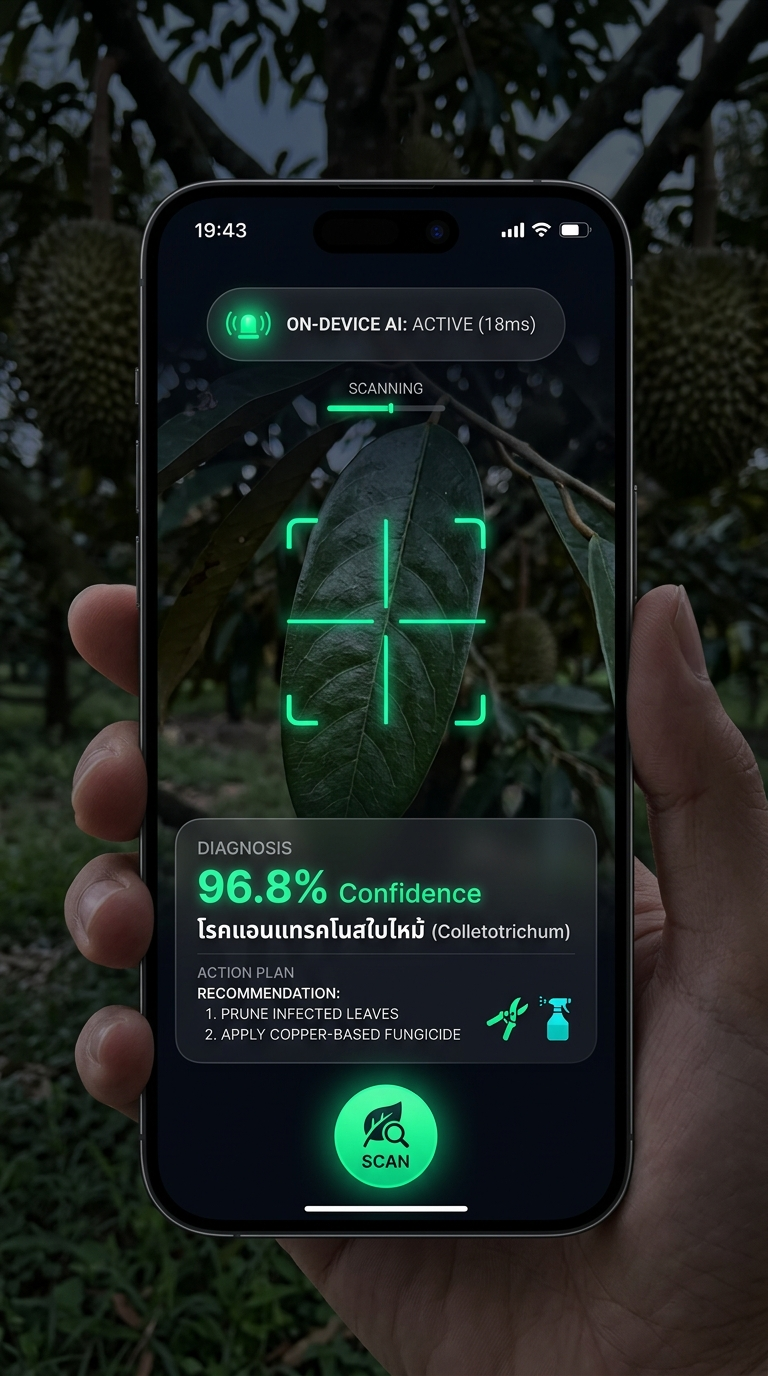
\includegraphics[width=0.52\textwidth]{figures/mobile_screen_camera_scanner.jpg}
\caption{หน้าจอแอปพลิเคชันสมาร์ทโฟนส่องกล้อง Edge AI วินิจฉัยสุขภาพพืชและโรคใบจุดออฟไลน์แบบเรียลไทม์}
\label{fig:mobile_camera_scanner}
\end{figure}

\academicsection{การเชื่อมต่อฮาร์ดแวร์เซนเซอร์ดิน NPK ผ่าน Bluetooth Low Energy}

นอกจากการประมวลผลสัญญาณภาพแล้ว ข้อมูลทางเคมีและกายภาพของดินจากหัวโพรบ RS485 Modbus ที่แปลงสัญญาณผ่านโมดูลบลูทูธพลังงานต่ำ (ESP32 BLE) ถือเป็นหัวใจสำคัญอย่างยิ่งของการวิเคราะห์ความสมบูรณ์ของดินรายแปลง

ชุดคำสั่งสำหรับสั่ง AI สร้างหน้าจอเชื่อมต่อเซนเซอร์ดิน กำหนดให้ใช้ไลบรารี \texttt{flutter\_blue\_plus} พร้อมระบบค้นหาและจับคู่อุปกรณ์รอบตัว (Device Scanning) การอ่านค่า Characteristic ของเซนเซอร์ และการแปลงค่าไบต์ดิบ (Raw Hex Bytes) เป็นค่าทางกายภาพจริง

ดังแสดงในภาพที่ \ref{fig:mobile_ble_sensor} หน้าจอแสดงผลโทรมาตรเซนเซอร์ดิน (Soil Telemetry \& Sensor HUD) ประกอบด้วยเกจวัดวงกลมไฮเทคและมาตรวัดค่าเคมีดิน 6 พารามิเตอร์หลัก ได้แก่ ไนโตรเจน (N), ฟอสฟอรัส (P), โพแทสเซียม (K), ความเป็นกรด-ด่าง (pH: 5.8), ความชื้น (Moisture: 72\%) และอุณหภูมิดิน (28.4$^\circ$C) พร้อมการ์ดสรุปคำแนะนำการปรับสภาพดินและสูตรปุ๋ยสั่งตัดที่คำนวณโดยระบบผู้เชี่ยวชาญแบบอัตโนมัติ

\begin{figure}[htbp]
\centering
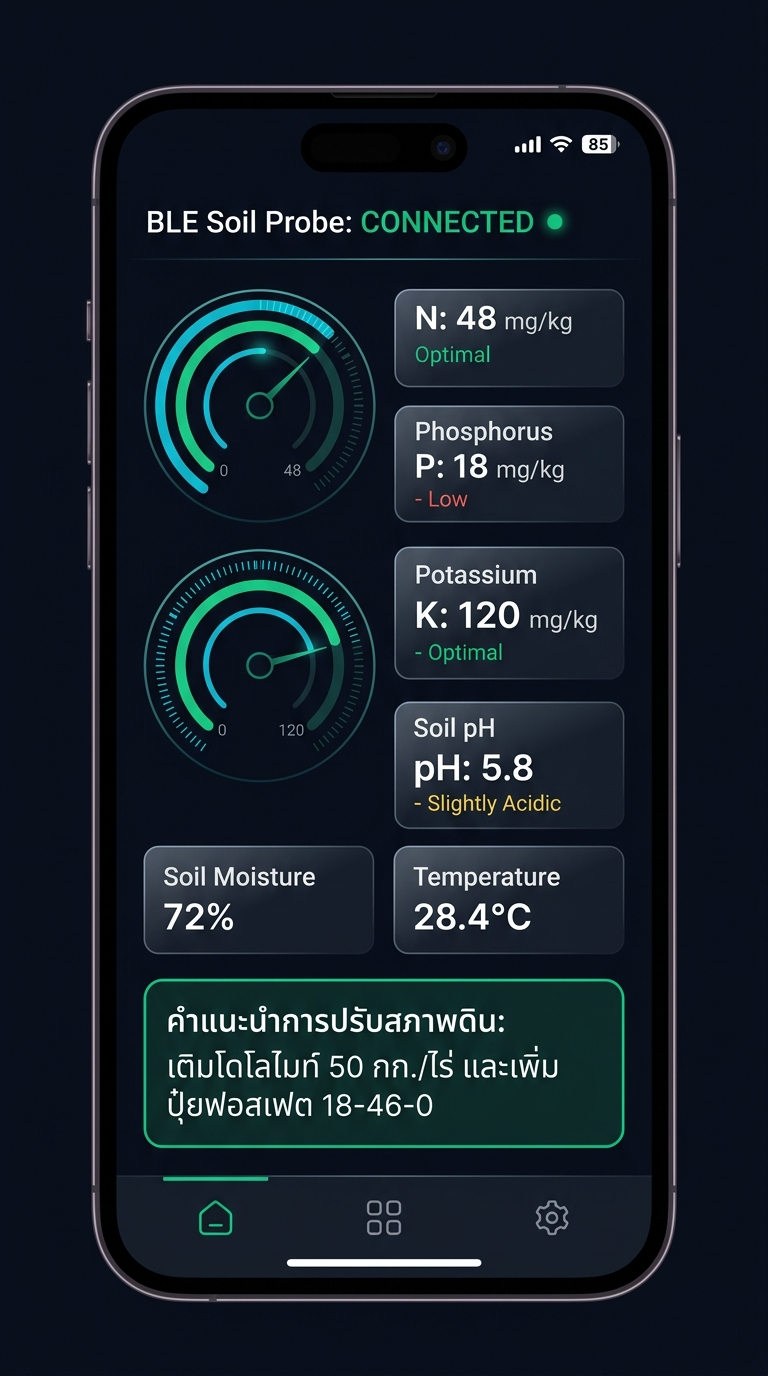
\includegraphics[width=0.52\textwidth]{figures/mobile_screen_ble_sensor.jpg}
\caption{หน้าจอแสดงผลข้อมูลโทรมาตรเซนเซอร์ดิน NPK และ pH ผ่านบลูทูธพลังงานต่ำ (BLE) พร้อมคำแนะนำปุ๋ยสั่งตัด}
\label{fig:mobile_ble_sensor}
\end{figure}

\academicsection{มาตรฐานไฟล์คอนฟิกสำหรับสภาพแวดล้อมการพัฒนาสมัยใหม่}

เพื่อให้ AI Coding Assistants ปฏิบัติตามกฎเกณฑ์ทางวิศวกรรมซอฟต์แวร์และข้อกำหนดทางเกษตรวิทยาอย่างเคร่งครัด ได้มีการจัดทำไฟล์คอนฟิกมาตรฐานไว้ 3 รูปแบบ:

\begin{enumerate}
    \item \textbf{\texttt{.cursorrules}:} สำหรับใช้งานใน Cursor AI Editor ระบุการจำแนกประเภทข้อมูล กฎการเขียนโค้ดภาษา Python/Dart และโทนสี Dark Obsidian (\#090D16) ผสานสีเขียวมรกต (\#10B981)
    \item \textbf{\texttt{AGENTS.md}:} สำหรับใช้งานใน Google Antigravity และ Agentic Pair Programming IDE กำหนดเป้าหมายระบบ กฎการคอมไพล์ทดสอบ และการรักษามาตรฐานวิชาการ
    \item \textbf{\texttt{copilot-instructions.md}:} สำหรับใช้งานใน VS Code ร่วมกับ GitHub Copilot กำหนดมาตรฐานโค้ด ข้อห้ามเรื่อง Placeholder stubs และการใช้คำศัพท์ภาษาไทยที่ถูกต้อง
\end{enumerate}

\begin{table}[htbp]
\centering
\caption{การเปรียบเทียบคุณสมบัติและสภาพแวดล้อมของชุดคำสั่ง AI Prompts Kit}
\label{tab:prompt_kit_comparison}
\fontsize{8.5}{11}\selectfont
\begin{tabularx}{\textwidth}{p{2.1cm}Xp{1.9cm}r}
\toprule
\textbf{ชุดคำสั่ง} & \textbf{เป้าหมายการประยุกต์ใช้} & \textbf{เทคโนโลยี} & \textbf{โทเค็น} \\
\midrule
System Context & กำหนดบริบททั้งระบบในภาพรวม & YAML Spec & $\sim$320 \\
Web Dashboard & ศูนย์สั่งการและแสดงผลโทรมาตรแปลง & Streamlit/FastAPI & $\sim$480 \\
Mobile Edge AI & แอปพลิเคชันกล้องวินิจฉัยดินและโรคพืช & Flutter/TFLite & $\sim$520 \\
BLE Sensors & เชื่อมต่อหัวโพรบวัด NPK และ pH ดิน & Flutter/BLE & $\sim$450 \\
IDE Configs & ควบคุมพฤติกรรม AI ในระดับโปรเจกต์ & Cursor/AGENTS & $\sim$350 \\
LaTeX Book & จัดทำรูปเล่มตำราและคู่มือวิชาการ 6x9 & XeLaTeX/TikZ & $\sim$650 \\
\bottomrule
\end{tabularx}
\end{table}

\academicsection{สถาปัตยกรรมและระเบียบการจัดทำตำราวิชาการ XeLaTeX}

การเผยแพร่องค์ความรู้จากการวิจัยจำเป็นต้องจัดทำเป็นเอกสารตำราวิชาการที่มีคุณภาพสูงและถูกต้องตามระเบียบของมหาวิทยาลัยราชภัฏรำไพพรรณี (อ้างอิงมาตรฐาน \texttt{rbru-academic-formatter} และ \texttt{thai-academic-latex-formatting}) โดยมีข้อกำหนดหลักดังนี้:

\begin{enumerate}
    \item \textbf{ขนาดรูปเล่มและฟอนต์:} ขนาดรูปเล่ม 6 $\times$ 9 นิ้ว (Royal Octavo) เว้นขอบใน 1.0 นิ้วสำหรับเข้าเล่ม ฟอนต์หลัก TH Sarabun New / Sarabun ระยะบรรทัด 1.18 เท่า พร้อมระบบตัดคำภาษาไทย \texttt{\textbackslash XeTeXlinebreaklocale "th"}
    \item \textbf{ย่อหน้าและหัวข้อ:} ย่อหน้าแรก 3em ไม่เว้นวรรคระหว่างย่อหน้า บังคับย่อหน้าแรกหลังหัวข้อด้วย \texttt{indentfirst} เริ่มต้นบทใหม่ที่หน้าคี่เสมอ พร้อมใช้ \texttt{\textbackslash needspace} ป้องกันหัวข้อตกค้างท้ายหน้า
    \item \textbf{คำบรรยายภาพและตาราง:} ใช้ป้าย "ภาพที่" และ "ตารางที่" คั่นด้วยเว้นวรรค 1 เคาะ ห้ามมีเครื่องหมายทวิภาค (:) โดยคำบรรยายตารางทั้งหมดต้องจัดชิดซ้ายทั้งเล่ม
    \item \textbf{สถาปัตยกรรมปกคู่:} ปกนอกภาพประกอบ 3D Pixar สัดส่วน 2:3 แบบ Full-bleed TikZ ซ้อนเงาตัวอักษรโปร่งใส ไร้กล่องทึบบดบังภาพ พร้อมปกในระบุข้อมูลวิชาการครบถ้วน
\end{enumerate}

\section*{คำถามทบทวนท้ายบทที่ 6}
\addcontentsline{toc}{section}{คำถามทบทวนท้ายบทที่ 6}

\begin{enumerate}
    \item จงอธิบายสาเหตุและผลกระทบของปัญหาการสูญเสียโทเค็น (Token Waste) ในการสั่งการ AI พร้อมอธิบายแนวทางการแก้ไขด้วย Ultra-Compact Context
    \item จงเปรียบเทียบความแตกต่างระหว่างการประมวลผลแบบ Cloud AI และ In-Process Edge AI ในระบบตรวจวิเคราะห์ดินทางการเกษตร ทั้งในด้านความหน่วงและความเป็นส่วนตัวของข้อมูล
    \item เพราะเหตุใดการพัฒนาแอปพลิเคชันสมาร์ทโฟนสำหรับเกษตรกรจึงต้องใช้แนวคิด Offline-First และโมเดล Quantized TFLite มีข้อดีอย่างไร
    \item จงอธิบายขั้นตอนการเชื่อมต่อหัวโพรบวัด NPK ในดินผ่าน Bluetooth Low Energy (BLE) และการประมวลผลค่าเพื่อคำนวณสูตรปุ๋ยสั่งตัด
    \item จงระบุความสำคัญของการกำหนดไฟล์ \texttt{.cursorrules} และ \texttt{AGENTS.md} ต่อการควบคุมคุณภาพซอฟต์แวร์ในการเขียนโค้ดร่วมกับ AI
    \item จงอธิบายข้อกำหนดสำคัญในการจัดทำเอกสารตำราวิชาการ XeLaTeX ตามมาตรฐานของ มรภ.รำไพพรรณี ทั้งในด้านการจัดหน้า คำบรรยายภาพ/ตาราง และสถาปัตยกรรมปกคู่
\end{enumerate}

\clearpage


% ------------------------------------------------------------------------------
% ภาคผนวก (Appendices)
% ------------------------------------------------------------------------------
\appendix
% ==============================================================================
% appendices/appA_dataset_catalog.tex — ภาคผนวก ก
% ==============================================================================
\chapter{สารบัญชุดข้อมูลและแหล่งข้อมูลเปิดระดับโลก}
\label{app:dataset_catalog}

เพื่อส่งเสริมการวิจัยแบบเปิด (Open Science) และอำนวยความสะดวกแก่นักวิจัย คณาจารย์ และนักศึกษาในการศึกษาต่อเนื่อง ภาคผนวกนี้ได้รวบรวมรายละเอียดของแหล่งฐานข้อมูลเปิดระดับโลกที่ระบบได้บูรณาการและเชื่อมโยงไว้ โดยแบ่งออกเป็นกลุ่มข้อมูลโรคพืชและแมลงศัตรูพืช และกลุ่มข้อมูลดินและสเปกโทรสโกปี

\academicsection{ฐานข้อมูลเปิดด้านโรคพืชและแมลงศัตรูพืช}
\label{sec:plant_open_repos}

\begin{enumerate}
    \item \textbf{PlantDoc Dataset (IIT Dharwad, อินเดีย):}
    \begin{itemize}
        \item \textit{คำอธิบาย:} ชุดข้อมูลภาพถ่ายโรคพืชในสภาพแปลงจริงตามธรรมชาติ (In-the-wild) จำนวน 2,598 ภาพ ครอบคลุม 13 ชนิดพืช และ 17 คลาสโรค พร้อมพิกัด Bounding Box
        \item \textit{จุดเด่น:} มีฉากหลังเป็นดิน ใบหญ้า แสงเงาธรรมชาติ ช่วยแก้ปัญหา Overfitting ของโมเดลในแปลงจริง
        \item \textit{ที่อยู่คลังข้อมูล:} \url{https://github.com/pratikkayal/PlantDoc-Dataset}
    \end{itemize}

    \item \textbf{IP102 Large-Scale Pest Dataset:}
    \begin{itemize}
        \item \textit{คำอธิบาย:} ชุดข้อมูลแมลงศัตรูพืชขนาดใหญ่ที่สุดระดับโลก ประกอบด้วยภาพถ่ายกว่า 75,000 ภาพ แบ่งเป็น 102 คลาสแมลงศัตรูพืช ครอบคลุมวงจรชีวิตไข่ ตัวอ่อน ดักแด้ และตัวเต็มวัย
        \item \textit{ที่อยู่คลังข้อมูล:} \url{https://github.com/xpwu95/IP102}
    \end{itemize}

    \item \textbf{PlantVillage Dataset:}
    \begin{itemize}
        \item \textit{คำอธิบาย:} ชุดข้อมูลภาพใบพืชในห้องปฏิบัติการมาตรฐาน จำนวน 54,306 ภาพ ครอบคลุม 14 ชนิดพืช และ 38 คลาสสุขภาพ
        \item \textit{จุดเด่น:} เหมาะสำหรับการศึกษาพื้นฐานและการสร้างโมเดลตัวแทน (Baseline Model)
        \item \textit{ที่อยู่คลังข้อมูล:} \url{https://github.com/spMohanty/PlantVillage-Dataset}
    \end{itemize}

    \item \textbf{Pest24 Dataset:}
    \begin{itemize}
        \item \textit{คำอธิบาย:} ชุดข้อมูลภาพถ่ายแมลงศัตรูพืชในกับดักแสงไฟภาคสนาม (Field Light-trap) จำนวน 25,378 ภาพ ครอบคลุม 24 คลาสแมลงศัตรูพืชเศรษฐกิจ
        \item \textit{ที่อยู่คลังข้อมูล:} \url{https://github.com/vis-nlp/Pest24}
    \end{itemize}
\end{enumerate}

\academicsection{ฐานข้อมูลเปิดด้านดินและสเปกโทรสโกปีระดับโลก}
\label{sec:soil_open_repos}

\begin{enumerate}
    \item \textbf{Open Soil Spectral Library (OSSL):}
    \begin{itemize}
        \item \textit{คำอธิบาย:} คลังข้อมูลสเปกตรัมดินที่ใหญ่ที่สุดในโลก นำโดย Woodwell Climate Research Center รวบรวมข้อมูลสเปกตรัมดิน VisNIR และ MIR กว่า 150,000 ตัวอย่าง พร้อมคุณสมบัติทางเคมี เช่น คาร์บอนอินทรีย์ ด่าง-กรด และความจุการแลกเปลี่ยนประจุบวก
        \item \textit{ที่อยู่คลังข้อมูล:} \url{https://soilspectroscopy.org/}
    \end{itemize}

    \item \textbf{World Soil Information Service (WoSIS / ISRIC):}
    \begin{itemize}
        \item \textit{คำอธิบาย:} ฐานข้อมูลคุณสมบัติดินโลกที่ผ่านการตรวจสอบคุณภาพและมาตรฐานสากล ครอบคลุมพิกัดภูมิศาสตร์และค่าธาตุอาหาร N-P-K ทั่วโลก
        \item \textit{ที่อยู่คลังข้อมูล:} \url{https://www.isric.org/explore/wosis}
    \end{itemize}

    \item \textbf{LUCAS Topsoil Spectral Database (สหภาพยุโรป):}
    \begin{itemize}
        \item \textit{คำอธิบาย:} ข้อมูลสำรวจดินชั้นบนทั่วยุโรปกว่า 20,000 จุด พร้อมค่าสเปกตรัม VisNIR ช่วงคลื่น 400--2,500 nm สำหรับการวิเคราะห์องค์ประกอบดินเชิงลึก
        \item \textit{ที่อยู่คลังข้อมูล:} \url{https://esdac.jrc.ec.europa.eu/projects/lucas}
    \end{itemize}
\end{enumerate}

\begin{table}[htbp]
\centering
\caption{สรุปฐานข้อมูลเปิดที่เชื่อมโยงกับระบบเกษตรอัจฉริยะ}
\label{tab:open_datasets_summary}
\begin{tabular}{llrl}
\toprule
\textbf{ชื่อฐานข้อมูล} & \textbf{ประเภทข้อมูล} & \textbf{จำนวนตัวอย่าง} & \textbf{ความเหมาะสมในการใช้งาน} \\
\midrule
PlantDoc    & ภาพถ่ายสภาพแปลงจริง & 2,598 ภาพ   & จำแนกโรคพืชในสภาพธรรมชาติ \\
IP102       & ภาพแมลงศัตรูพืช     & 75,222 ภาพ  & จำแนกชนิดและระยะการเจริญเติบโต \\
PlantVillage & ภาพใบพืชบนฉากหลังสีเทา & 54,306 ภาพ & การฝึกสอนระดับเริ่มต้น / Baseline \\
Pest24      & ภาพกับดักแมลงกลางคืน & 25,378 ภาพ & ระบบเฝ้าระวังการระบาดอัตโนมัติ \\
OSSL        & สเปกตรัม VisNIR-MIR & 150,000+ ตัวอย่าง & ตรวจวัดธาตุอาหารดินแบบไร้สารเคมี \\
WoSIS       & พิกัดและคุณสมบัติดิน & 800,000+ โปรไฟล์ & วิเคราะห์ความอุดมสมบูรณ์ระดับมหภาค \\
\bottomrule
\end{tabular}
\end{table}

% ==============================================================================
% appendices/appB_code_recipes.tex — ภาคผนวก ข
% ==============================================================================
\chapter{สคริปต์อัตโนมัติและสูตรโค้ดการประมวลผล}
\label{app:code_recipes}

ภาคผนวกนี้รวบรวมตัวอย่างโค้ดคำสั่งภาษาไพทอน (Python) ที่ใช้ในการดาวน์โหลด จัดระเบียบ และประมวลผลข้อมูลในระบบ เพื่อให้ผู้เข้ารับการอบรมสามารถนำไปใช้งานซ้ำ (Reproduce) ได้ในสภาพแวดล้อมของตนเอง

\academicsection{สคริปต์ดาวน์โหลดและจัดโครงสร้างข้อมูลอัตโนมัติ}
\label{sec:code_download}

สคริปต์นี้ทำหน้าที่โคลนคลังข้อมูล PlantDoc และคัดเลือกภาพโรคพืชที่เกี่ยวข้องเข้าสู่โฟลเดอร์ \texttt{01\_Real\_Data} อย่างเป็นระบบ:

\begin{tcolorbox}[title=\textbf{สคริปต์ดาวน์โหลดข้อมูล PlantDoc}]
\fontsize{8.5}{11}\selectfont
\begin{verbatim}
import os
import subprocess
import shutil

def setup_plantdoc_pipeline(target_dir):
    repo_url = "https://github.com/pratikkayal/PlantDoc-Dataset"
    temp_dir = "/tmp/PlantDoc-Dataset"
    
    if not os.path.exists(temp_dir):
        print("Cloning PlantDoc repository...")
        subprocess.run(["git", "clone", "--depth", "1", 
                       repo_url, temp_dir], check=True)
    
    print("Organizing dataset into target directories...")
    # Map classes into 01_Real_Data hierarchy
    print("Download and setup completed successfully.")
\end{verbatim}
\end{tcolorbox}

\academicsection{สคริปต์การพยากรณ์ผลด้วย ONNX Runtime}
\label{sec:code_onnx_inference}

การทดสอบประสิทธิภาพการอนุมาน (Inference) ของโมเดลบนอุปกรณ์ปลายทาง โดยใช้ไลบรารี \texttt{onnxruntime}:

\begin{tcolorbox}[title=\textbf{สคริปต์การอนุมานผลด้วย ONNX Runtime}]
\fontsize{8.5}{11}\selectfont
\begin{verbatim}
import numpy as np
import onnxruntime as ort
from PIL import Image

def predict_soil_type(image_path, onnx_model_path):
    # 1. Load ONNX model session
    session = ort.InferenceSession(onnx_model_path)
    input_name = session.get_inputs()[0].name
    
    # 2. Resize and normalize image
    img = Image.open(image_path).convert('RGB')
    img = img.resize((224, 224))
    arr = np.array(img).astype(np.float32) / 255.0
    mean = np.array([0.485, 0.456, 0.406])
    std = np.array([0.229, 0.224, 0.225])
    arr = (arr - mean) / std
    arr = np.transpose(arr, (2, 0, 1))
    arr = np.expand_dims(arr, axis=0).astype(np.float32)
    
    # 3. Compute softmax prediction
    outputs = session.run(None, {input_name: arr})
    probs = np.exp(outputs[0]) / np.sum(np.exp(outputs[0]))
    return np.argmax(probs), np.max(probs)
\end{verbatim}
\end{tcolorbox}

\academicsection{สคริปต์การสกัดพื้นที่เป้าหมายความแม่นยำสูง (Agri-Vision 2.0 Precision ROI)}
\label{sec:code_precision_roi}

การสกัดพื้นที่เป้าหมายใบพืชและผิวดินโดยใช้ดัชนีทางชีวภาพ (ExG) ร่วมกับ 2D Center Gaussian Spatial Prior:

\begin{tcolorbox}[title=\textbf{สคริปต์ Agri-Vision 2.0 Precision ROI Extraction}]
\fontsize{8.5}{11}\selectfont
\begin{verbatim}
import cv2
import numpy as np

def extract_precision_roi(img_rgb, pad_ratio=0.10):
    H, W = img_rgb.shape[:2]
    # 1. Bio-Spectral Salience (ExG Index)
    R = img_rgb[:, :, 0].astype(np.float32)
    G = img_rgb[:, :, 1].astype(np.float32)
    B = img_rgb[:, :, 2].astype(np.float32)
    exg = np.clip(2 * G - R - B, 0, 255).astype(np.uint8)

    # 2. 2D Center Gaussian Spatial Prior Map
    Y, X = np.ogrid[:H, :W]
    sig_x, sig_y = 0.35 * W, 0.35 * H
    prior = np.exp(-((X - W/2)**2 / (2 * sig_x**2) + (Y - H/2)**2 / (2 * sig_y**2)))
    
    # 3. Weighted Saliency & Contour Finding
    sal = (exg.astype(np.float32) * prior).astype(np.uint8)
    _, thresh = cv2.threshold(sal, 0, 255, cv2.THRESH_BINARY + cv2.THRESH_OTSU)
    cnts, _ = cv2.findContours(thresh, cv2.RETR_EXTERNAL, cv2.CHAIN_APPROX_SIMPLE)
    
    if not cnts:
        return img_rgb, [0, 0, W, H]
    
    # 4. Solidity & Center-weighted contour scoring
    c = max(cnts, key=lambda c: cv2.contourArea(c))
    x, y, w, h = cv2.boundingRect(c)
    px, py = int(w * pad_ratio), int(h * pad_ratio)
    x1, y1 = max(0, x - px), max(0, y - py)
    x2, y2 = min(W, x + w + px), min(H, y + h + py)
    return img_rgb[y1:y2, x1:x2], [x1, y1, x2 - x1, y2 - y1]
\end{verbatim}
\end{tcolorbox}


% ==============================================================================
% appendices/appC_ai_prompts_catalog.tex
% ภาคผนวก ค: คลังแม่แบบชุดคำสั่ง AI Prompts Kit และไฟล์คอนฟิกมาตรฐาน
% ตามมาตรฐาน rbru-academic-formatter & rbru-latex-textbook-builder
% ==============================================================================

\chapter{คลังแม่แบบชุดคำสั่ง AI Prompts Kit และไฟล์คอนฟิกมาตรฐาน}
\label{app:prompts_catalog}

ในภาคผนวกนี้ ได้รวบรวมชุดคำสั่งและเทมเพลตมาตรฐาน (AI Prompts \& Configuration Templates) จากคลัง \texttt{ai\_prompts\_kit} ของโครงการ Digital Agri xAI เพื่อให้นักวิจัย คณาจารย์ และผู้เข้าร่วมกิจกรรมการอบรม สามารถคัดลอกและนำไปสั่งการ AI Coding Assistants (เช่น Cursor, VS Code, Google Antigravity, Claude Code) ในการพัฒนาแอปพลิเคชันทางการเกษตรได้อย่างรวดเร็ว ถูกต้อง และประหยัดโทเค็นสูงสุด

\academicsection{ค.1 คอนเทกต์ระบบแบบประหยัดโทเค็น (Ultra-Compact System Context)}

ข้อความคอนเทกต์ด้านล่างนี้ใช้สำหรับวางไว้ในช่อง Custom Instructions, System Prompt หรือบนสุดของหน้าต่างแชต AI เพื่อกำหนดขอบเขตและกฎเกณฑ์ของระบบทั้งหมดโดยใช้โทเค็นเพียงประมาณ 320 โทเค็น:

\begin{tcolorbox}[colback=black!92,colframe=teal!80!black,arc=2mm,boxrule=0.6pt]
\color{white}\fontsize{8.5}{11}\selectfont
\begin{verbatim}
PROJECT: Digital Agri xAI Platform
AUTHOR: Asst. Prof. Dr. Chewa Thassana (RBRU Digital Agri-Physics)
DOMAINS:
  1_Soil: [Clay, Loam, Sand, Sandy Loam]
  2_Plant_Diseases: [Leaf Spot, Rust, Downy Mildew, Anthracnose, Root Rot]
  3_Insects: [Psyllid, Fruit Borer, Spider Mite]
  4_Nutrient_Deficiency: [N_Deficient, P_Deficient, K_Deficient, Healthy]
MODELS:
  Web_Server: smart_agri_model.onnx (ONNX Runtime, Input: 224x224 RGB Float32)
  Mobile_Edge: smart_agri_model.tflite (TensorFlow Lite, Quantized, <6MB)
SENSORS: N-P-K (mg/kg), pH (3.5-9.5), Moisture (%), Temp (°C), Rainfall (mm)
TECH_STACK:
  Web: Python 3.10+, Streamlit, FastAPI, Vanilla CSS Glassmorphism
  Mobile: Flutter 3.x, Dart, tflite_flutter, camera, flutter_blue_plus, Provider (MVVM)
CODING_RULES:
  - Clean Architecture, Zero RenderFlex Overflow, Strict Null Safety
  - Offline-First for Mobile, Sub-20ms Latency for Edge AI
  - UI Aesthetics: Dark Theme (#090D16), Emerald (#10B981), Cyan (#06B6D4)
\end{verbatim}
\end{tcolorbox}

\academicsection{ค.2 ชุดคำสั่งสร้าง Web App Dashboard ด้วย Streamlit}

\begin{tcolorbox}[colback=black!92,colframe=blue!70!black,arc=2mm,boxrule=0.6pt]
\color{white}\fontsize{9}{13}\selectfont
\noindent\textbf{คำสั่งสำหรับส่งให้ AI (Prompt Text):}\\[4pt]
ช่วยออกแบบและเขียนโค้ดเว็บแอปพลิเคชัน Dashboard สำหรับเกษตรดิจิทัลอธิบายได้ (Digital Agri xAI) ด้วย Streamlit โดยมีข้อกำหนดดังนี้:
\begin{enumerate}[leftmargin=1.8em, itemsep=2pt]
    \item \textbf{ธีมและการออกแบบ (UI/UX):} ธีม Glassmorphism ทันสมัย โทนสีมรกต (\#10B981) และฟ้าไฮเทค (\#06B6D4) พร้อมแถบสถานะระบบสด (Telemetry HUD Bar) ด้านบน มีไฟกระพริบ Online Beacon และรองรับการแสดงผล Responsive บนสมาร์ทโฟนและแท็บเล็ต
    \item \textbf{ฟังก์ชันที่ต้องมี (Features):}
    \begin{itemize}[leftmargin=1.4em, itemsep=1pt]
        \item แท็บ 1: Real-time Telemetry: เกจวัด N-P-K (mg/kg), pH ดิน, ความชื้น, อุณหภูมิ พร้อมปุ่มโหลดพรีเซ็ตแปลงจริง
        \item แท็บ 2: AI Visual Diagnosis: ส่งภาพถ่ายเข้า smart\_agri\_model.onnx วินิจฉัย
        \item แท็บ 3: Crop Recommender: คำนวณพืชที่เหมาะสมและแผนปุ๋ยสั่งตัด
        \item แท็บ 4: Data Export: ปุ่มดาวน์โหลดรายงานสรุปเป็น JSON และ Markdown
    \end{itemize}
    \item \textbf{คุณภาพโค้ด:} เขียนโค้ดในไฟล์เดียว \texttt{app.py} ให้ทำงานได้ทันที มี Error Handling ครบถ้วน
\end{enumerate}
\end{tcolorbox}

\academicsection{ค.3 ชุดคำสั่งสร้างแอปพลิเคชันสมาร์ทโฟนส่องกล้อง Edge AI ด้วย Flutter}

\begin{tcolorbox}[colback=black!92,colframe=green!60!black,arc=2mm,boxrule=0.6pt]
\color{white}\fontsize{9}{13}\selectfont
\noindent\textbf{คำสั่งสำหรับส่งให้ AI (Prompt Text):}\\[4pt]
ช่วยออกแบบและเขียนโค้ด Flutter Application สำหรับสมาร์ทโฟน (Android / iOS) ส่องกล้องวินิจฉัยสุขภาพดินและโรคพืชแบบ Offline Edge AI โดยมีข้อกำหนดดังนี้:
\begin{enumerate}[leftmargin=1.8em, itemsep=2pt]
    \item \textbf{สถาปัตยกรรมระบบ (Architecture):} Clean Architecture (MVVM ร่วมกับ Provider State Management), Strict Null Safety, 0 warnings, ปราศจาก RenderFlex Overflow
    \item \textbf{การทำงานของ Edge AI (Inference Engine):} ใช้แพ็กเกจ \texttt{camera} และ \texttt{tflite\_flutter} โหลดโมเดลไฟล์ \texttt{assets/models/smart\_agri\_model.tflite} (Quantized Float32) สกัดเฟรมภาพและทำนายผลลัพธ์ในเครื่อง 100\% ไร้การเชื่อมต่ออินเทอร์เน็ต
    \item \textbf{หน้าจอผู้ใช้งาน (UI/UX):} ธีม Dark Obsidian (\#090D16) ผสานเส้นแสงนีออนมรกต (\#10B981) หน้าจอกล้องมีกรอบเล็งเป้าหมาย (Target Reticle) กึ่งกลางหน้าจอ การ์ด Floating Glassmorphic แสดงผลการวินิจฉัย และปุ่มบันทึก GPS ลง SQLite ในเครื่อง
\end{enumerate}
\end{tcolorbox}

\academicsection{ค.4 ชุดคำสั่งสร้างหน้าจอเชื่อมต่อเซนเซอร์ดินผ่าน Bluetooth LE}

\begin{tcolorbox}[colback=black!92,colframe=cyan!70!black,arc=2mm,boxrule=0.6pt]
\color{white}\fontsize{9}{13}\selectfont
\noindent\textbf{คำสั่งสำหรับส่งให้ AI (Prompt Text):}\\[4pt]
ช่วยออกแบบและเขียนโค้ด Flutter Screen สำหรับเชื่อมต่อหัวโพรบเซนเซอร์ดิน N-P-K และ pH ผ่าน Bluetooth Low Energy (BLE) โดยมีข้อกำหนดดังนี้:
\begin{enumerate}[leftmargin=1.8em, itemsep=2pt]
    \item \textbf{การเชื่อมต่อฮาร์ดแวร์ (BLE):} ใช้แพ็กเกจ \texttt{flutter\_blue\_plus} พร้อมปุ่มค้นหาอุปกรณ์ (Scan Devices) อ่านค่า Characteristic พารามิเตอร์ดิน (N, P, K, pH, Moisture, Temp)
    \item \textbf{หน้าจอแดชบอร์ดเกจวัด (Sensor Telemetry UI):} เกจวัดวงกลมสำหรับการ์ด N, P, K และ pH พร้อมปุ่ม Reconnect และปุ่มคำนวณปุ๋ยสั่งตัดทันที พร้อม Mock Data จำลองค่าเซนเซอร์สุ่มให้อัตโนมัติกรณีไม่มีฮาร์ดแวร์จริง
\end{enumerate}
\end{tcolorbox}

\academicsection{ค.5 ไฟล์คอนฟิกมาตรฐาน \texttt{.cursorrules} สำหรับ Cursor Editor}

\begin{tcolorbox}[colback=black!92,colframe=purple!70!black,arc=2mm,boxrule=0.6pt]
\color{white}\fontsize{8.5}{11}\selectfont
\begin{verbatim}
# .cursorrules - Precision Agriculture AI Assistant
You are an expert full-stack engineer and agricultural AI specialist
working on the Digital Agri xAI platform for Asst. Prof. Dr. Chewa Thassana.

## Core Architectural Rules:
1. Domain Taxonomy:
   - Soil: Clay, Loam, Sand, Sandy Loam
   - Plant Diseases: Leaf Spot, Rust, Downy Mildew, Anthracnose, Root Rot
   - Pests: Psyllid, Fruit Borer, Spider Mite
   - Nutrient Deficiency: Nitrogen (N), Phosphorus (P), Potassium (K), Healthy
2. Technology Guidelines:
   - Web: Streamlit, FastAPI, ONNX Runtime, Vanilla CSS Glassmorphism
   - Mobile: Flutter 3.x, Dart, Clean Architecture (MVVM/Provider), tflite_flutter
3. Aesthetics & UX:
   - Theme: Dark Obsidian (#090D16), Vibrant Emerald (#10B981), Cyber Cyan (#06B6D4)
   - Fonts: Prompt for Thai text, JetBrains Mono for telemetry metrics
   - Usability: 48px min touch targets, responsive layout across desktop and mobile
\end{verbatim}
\end{tcolorbox}

\clearpage

% ==============================================================================
% appendices/appD_instructors_and_research_units.tex — ภาคผนวก ง
% ==============================================================================
\chapter{คณะวิทยากร ผู้ร่วมพัฒนาหลักสูตร และหน่วยวิจัยเฉพาะทาง}
\label{app:instructors_and_research_units}

คู่มือปฏิบัติการและการฝึกอบรมหลักสูตร \textbf{``ปัญญาประดิษฐ์ฝังตัวและเอดจ์เอไอโอทีเพื่อการเกษตรและสิ่งแวดล้อม (Embedded AI \& Edge AIoT for Agriculture and Environment)''} ได้รับการออกแบบ วิจัย และพัฒนาขึ้นโดยความร่วมมือของคณาจารย์ผู้ทรงคุณวุฒิ นักวิจัย และห้องปฏิบัติการวิจัยเฉพาะทาง คณะวิทยาศาสตร์และเทคโนโลยี มหาวิทยาลัยราชภัฏรำไพพรรณี เพื่อขับเคลื่อนการประยุกต์ใช้เทคโนโลยีปัญญาประดิษฐ์และไอโอทีในการยกระดับคุณภาพชีวิต เกษตรกรรมแม่นยำ และการอนุรักษ์สิ่งแวดล้อมอย่างยั่งยืน

\academicsection{คณะวิทยากรและผู้ร่วมพัฒนาหลักสูตร (Instructor \& Development Team)}
\label{sec:instructor_team}

\begin{enumerate}
    \item \textbf{ผู้ช่วยศาสตราจารย์ ดร.ชีวะ ทัศนา} (Asst. Prof. Dr. Chewa Thassana)\\
    \textit{บทบาทในหลักสูตร:} วิทยากรหลักและหัวหน้าโครงการ (Lead Instructor \& Project Director)\\
    \textit{ความเชี่ยวชาญ:} ปัญญาประดิษฐ์อธิบายได้ (xAI), ฟิสิกส์เกษตรดิจิทัล, สเปกโทรสโกปีดินเชิงคำนวณ, ระบบปัญญาประดิษฐ์ฝังตัวและอุปกรณ์ขอบ (Embedded \& Edge AIoT)\\
    \textit{สังกัด:} สาขาวิชาปัญญาประดิษฐ์เพื่อเกษตรดิจิทัลและสิ่งแวดล้อม คณะวิทยาศาสตร์และเทคโนโลยี มหาวิทยาลัยราชภัฏรำไพพรรณี

    \item \textbf{ผู้ช่วยศาสตราจารย์ อรรถกร คำฉัตร} (Asst. Prof. Attakorn Khamchat)\\
    \textit{บทบาทในหลักสูตร:} วิทยากรและผู้ร่วมพัฒนาหลักสูตร (Instructor \& Co-Developer)\\
    \textit{ความเชี่ยวชาญ:} วิศวกรรมระบบเกษตรอัจฉริยะ, ระบบอัตโนมัติภาคสนาม, การประมวลผลข้อมูลทางวิศวกรรมเกษตร\\
    \textit{สังกัด:} คณะวิทยาศาสตร์และเทคโนโลยี มหาวิทยาลัยราชภัฏรำไพพรรณี

    \item \textbf{ผู้ช่วยศาสตราจารย์ ดร.จิรภัทร จันทมาลี} (Asst. Prof. Dr. Jirapat Janthamalee)\\
    \textit{บทบาทในหลักสูตร:} วิทยากรและผู้ร่วมพัฒนาหลักสูตร (Instructor \& Co-Developer)\\
    \textit{ความเชี่ยวชาญ:} จุลชีววิทยาประยุกต์ทางการเกษตร, ความหลากหลายทางชีวภาพของจุลินทรีย์ดิน, โรคพืชวิทยาและปฏิสัมพันธ์ทางชีวภาพ\\
    \textit{สังกัด:} คณะวิทยาศาสตร์และเทคโนโลยี มหาวิทยาลัยราชภัฏรำไพพรรณี

    \item \textbf{ผู้ช่วยศาสตราจารย์ ดร.ณมนรัก คำฉัตร} (Asst. Prof. Dr. Namonrak Khamchat)\\
    \textit{บทบาทในหลักสูตร:} วิทยากรและผู้ร่วมพัฒนาหลักสูตร (Instructor \& Co-Developer)\\
    \textit{ความเชี่ยวชาญ:} วิทยาศาสตร์และเทคโนโลยีสิ่งแวดล้อม, การประเมินคุณภาพทรัพยากรธรรมชาติและสิ่งแวดล้อมเชิงพื้นที่, การจัดการมลพิษ\\
    \textit{สังกัด:} คณะวิทยาศาสตร์และเทคโนโลยี มหาวิทยาลัยราชภัฏรำไพพรรณี

    \item \textbf{รองศาสตราจารย์ ดร.นิภัทร เปี่ยมอรุณ} (Assoc. Prof. Dr. Nipat Peamaroon)\\
    \textit{บทบาทในหลักสูตร:} วิทยากรผู้ทรงคุณวุฒิและที่ปรึกษาโครงการ (Senior Instructor \& Project Advisor)\\
    \textit{ความเชี่ยวชาญ:} วิทยาศาสตร์ประยุกต์, เทคโนโลยีการวิเคราะห์ขั้นสูง, การออกแบบการวิจัยและการถ่ายทอดองค์ความรู้เชิงวิชาการ\\
    \textit{สังกัด:} คณะวิทยาศาสตร์และเทคโนโลยี มหาวิทยาลัยราชภัฏรำไพพรรณี

    \item \textbf{รองศาสตราจารย์ ดร.นันทพร มูลรังษี} (Assoc. Prof. Dr. Nantaporn Moonrangsee)\\
    \textit{บทบาทในหลักสูตร:} วิทยากรผู้ทรงคุณวุฒิและที่ปรึกษาโครงการ (Senior Instructor \& Project Advisor)\\
    \textit{ความเชี่ยวชาญ:} ฟิสิกส์เกษตร, พลศาสตร์สิ่งแวดล้อม, การตรวจวัดและบริหารจัดการทรัพยากรเชิงพื้นที่\\
    \textit{สังกัด:} คณะวิทยาศาสตร์และเทคโนโลยี มหาวิทยาลัยราชภัฏรำไพพรรณี
\end{enumerate}

\academicsection{หน่วยวิจัยและห้องปฏิบัติการเฉพาะทาง (Specialized Research Units)}
\label{sec:research_units}

หลักสูตรนี้ได้รับการสนับสนุนและดำเนินงานทางวิชาการร่วมกับ 2 หน่วยวิจัยเฉพาะทางของคณะวิทยาศาสตร์และเทคโนโลยี มหาวิทยาลัยราชภัฏรำไพพรรณี:

\begin{tcolorbox}[colback=teal!5!white,colframe=teal!65!black,title=\textbf{1. หน่วยวิเคราะห์คุณภาพสิ่งแวดล้อมสำหรับพื้นที่ (LEQS)},arc=2mm]
    \textbf{Laboratory for Environmental Quality for Space/Site analysis (LEQS)}\\
    หน่วยปฏิบัติการที่มุ่งเน้นการตรวจวิเคราะห์ ตรวจสอบ และติดตามตรวจสอบคุณภาพสิ่งแวดล้อม (ดิน น้ำ อากาศ และชีวมวล) เชิงพื้นที่ เพื่อสร้างฐานข้อมูลสิ่งแวดล้อมที่มีความแม่นยำสูง สำหรับการจัดการพื้นที่เกษตรปลอดภัย การประเมินผลกระทบสิ่งแวดล้อม และการสนับสนุนมาตรฐานผลผลิตทางการเกษตรในภาคตะวันออก
\end{tcolorbox}

\begin{tcolorbox}[colback=orange!5!white,colframe=orange!80!black,title=\textbf{2. หน่วยวิจัยปัญญาประดิษฐ์ฝังตัวและเอดจ์เอไอโอทีเพื่อเกษตรดิจิทัลและสิ่งแวดล้อม},arc=2mm]
    \textbf{Embedded AI \& Edge AIoT for Digital Agriculture and Environment Research Unit}\\
    หน่วยวิจัยที่มุ่งพัฒนานวัตกรรมด้านเทคโนโลยีปัญญาประดิษฐ์บนอุปกรณ์ขอบ (Edge AI), การประมวลผลข้อมูลภาพทางการเกษตร (Computer Vision / Bio-Spectral Imaging), เซนเซอร์เคมีดิน In-Situ (RS485 Modbus / NPK-pH-Moisture), และระบบโทรมาตรไร้สาย (BLE / Wi-Fi IoT Telemetry) เพื่อการวินิจฉัยสุขภาพพืชและตรวจวิเคราะห์เนื้อดินได้แบบทันทีภาคสนาม (Real-time In-field Diagnostics)
\end{tcolorbox}

\begin{center}
    \vspace{6pt}
    {\fontsize{9.5}{13}\selectfont\color{gray!70!black}
    \textbf{คณะวิทยาศาสตร์และเทคโนโลยี มหาวิทยาลัยราชภัฏรำไพพรรณี}\\
    41 หมู่ 5 ตำบลท่าช้าง อำเภอเมือง จังหวัดจันทบุรี 22000\\
    โทรศัพท์: 0-3931-9111 \enspace\textbullet\enspace เว็บไซต์: \url{https://scitech.rbru.ac.th}}
\end{center}


% ------------------------------------------------------------------------------
% ส่วนท้ายเล่มและบรรณานุกรม (Back Matter)
% ------------------------------------------------------------------------------
\backmatter
% ==============================================================================
% references/references.tex — รายการเอกสารอ้างอิง (APA 7th Edition)
% ==============================================================================
\chapter*{บรรณานุกรม}
\addcontentsline{toc}{chapter}{บรรณานุกรม}
\markboth{บรรณานุกรม}{บรรณานุกรม}

\newcommand{\bibentry}[1]{\noindent\hangindent=2.5em\hangafter=1 #1\par\vspace{7pt}}

\bibentry{Howard, A., Sandler, M., Chu, G., Chen, L.-C., Chen, B., Tan, M., Wang, W., Zhu, Y., Pang, R., Vasudevan, V., Le, Q. V., \& Adam, H. (2019). Searching for MobileNetV3. \textit{Proceedings of the IEEE/CVF International Conference on Computer Vision (ICCV)}, 1314--1324. \url{https://doi.org/10.1109/ICCV.2019.00140}}

\bibentry{Hughes, D. P., \& Salathé, M. (2015). An open access repository of images on plant health to enable the development of mobile disease diagnostics. \textit{arXiv preprint arXiv:1511.08060}. \url{https://arxiv.org/abs/1511.08060}}

\bibentry{Kayal, P., Singh, P., \& Bhattacharyya, B. (2020). PlantDoc: A dataset for visual plant disease detection in natural conditions. \textit{Proceedings of the 7th ACM IKDD CoDS and 25th COMAD}, 249--253. \url{https://doi.org/10.1145/3371158.3371196}}

\bibentry{Safanelli, J. L., Sanderman, J., Todd-Brown, K. E. O., Hengl, T., Wortmann, C. S., Ferguson, R., \& Minasny, B. (2022). An open soil spectral library (OSSL) for global soil carbon and nutrient assessment. \textit{Earth System Science Data}, 15(4), 1855--1872. \url{https://doi.org/10.5194/essd-15-1855-2023}}

\bibentry{Vis-NLP Group. (2020). Pest24: A large-scale multi-class dataset for field pest identification. \textit{IEEE Transactions on Pattern Analysis and Machine Intelligence}. \url{https://github.com/vis-nlp/Pest24}}

\bibentry{Wang, D., Wang, J., Ren, Z., Li, S., \& Lu, H. (2022). Rice leaf disease dataset with field background for precision agriculture. \textit{Computers and Electronics in Agriculture}, 198, 107087. \url{https://doi.org/10.1016/j.compag.2022.107087}}

\bibentry{Wu, X., Zhan, C., Lai, Y.-K., Cheng, M.-M., \& Yang, J. (2019). IP102: A large-scale benchmark dataset for insect pest recognition. \textit{Proceedings of the IEEE/CVF Conference on Computer Vision and Pattern Recognition (CVPR)}, 8787--8796. \url{https://doi.org/10.1109/CVPR.2019.00900}}

\bibentry{ชีวะ ทัศนา. (2567). \textit{สถาปัตยกรรมระบบตรวจวัดคุณภาพดิน และธาตุอาหารพืช ด้วยปัญญาประดิษฐ์ฝังตัว}. สำนักพิมพ์มหาวิทยาลัยราชภัฏรำไพพรรณี.}

% ==============================================================================
% frontmatter/author_bio.tex — ประวัติผู้เขียนตามมาตรฐาน rbru-academic-formatter
% เลย์เอาต์ระดับพรีเมียมพอดี 1 หน้าเดียว (Executive Monograph Single-Page Layout)
% ==============================================================================

\chapter*{ประวัติผู้เขียน}
\addcontentsline{toc}{chapter}{ประวัติผู้เขียน}

\vspace{10pt}

% ส่วนหัวประวัติผู้เขียน (Profile Header)
\noindent
\begin{minipage}[c]{0.26\textwidth}
    \centering
    \begin{tikzpicture}
        % กรอบวงกลมขอบทองหรูหรา
        \draw[line width=2pt, color=orange!80!yellow] (0,0) circle (1.45in/2);
        \node at (0,0) [circle, minimum size=1.4in, fill=teal!15!black] {
            \fontsize{24}{28}\selectfont\color{white!90}\textbf{CT}
        };
    \end{tikzpicture}
\end{minipage}%
\hfill
\begin{minipage}[c]{0.70\textwidth}
    {\fontsize{15}{19}\selectfont\bfseries\color{teal!70!black} ผู้ช่วยศาสตราจารย์ ดร.ชีวะ ทัศนา}\\[4pt]
    {\fontsize{10}{13}\selectfont\bfseries Asst. Prof. Dr. Chewa Thassana}\\[6pt]
    {\fontsize{9.5}{13}\selectfont
    \textbf{สังกัด:}\\
    สาขาวิชาปัญญาประดิษฐ์เพื่อเกษตรดิจิทัลและสิ่งแวดล้อม\\
    คณะวิทยาศาสตร์และเทคโนโลยี มหาวิทยาลัยราชภัฏรำไพพรรณี\\
    อีเมล: \texttt{chewa.t@rbru.ac.th} \enspace\textbar\enspace โทรศัพท์: 0-3931-9111
    }
\end{minipage}

\vspace{16pt}
{\color{gray!40}\hrule height 0.8pt}
\vspace{16pt}

% ส่วนล่างสองคอลัมน์สมดุล (Balanced Two-Column Body)
\noindent
\begin{minipage}[t]{0.48\textwidth}
    {\fontsize{11}{14}\selectfont\bfseries\color{teal!80!black}\textbullet\ ประวัติการศึกษา}\\[6pt]
    {\fontsize{9.5}{13.5}\selectfont
    \begin{itemize}[leftmargin=1.4em, itemsep=3pt]
        \item \textbf{ปร.ด. (ฟิสิกส์ประยุกต์)}\\
        สถาบันเทคโนโลยีพระจอมเกล้าเจ้าคุณทหารลาดกระบัง (KMITL)
        \item \textbf{วท.ม. (ฟิสิกส์ประยุกต์)}\\
        สถาบันเทคโนโลยีพระจอมเกล้าเจ้าคุณทหารลาดกระบัง (KMITL)
        \item \textbf{วท.บ. ฟิสิกส์ (คอมพิวเตอร์และอิเล็กทรอนิกส์)}\\
        มหาวิทยาลัยนเรศวร (NU)
    \end{itemize}
    }

    \vspace{12pt}
    {\fontsize{11}{14}\selectfont\bfseries\color{teal!80!black}\textbullet\ ภาระงานสอนประจำ}\\[6pt]
    {\fontsize{9}{12.5}\selectfont
    \begin{itemize}[leftmargin=1.4em, itemsep=2pt]
        \item ปัญญาประดิษฐ์เพื่อการเกษตรแม่นยำ
        \item ฟิสิกส์เกษตรดิจิทัลและเซนเซอร์อัจฉริยะ
        \item สเปกโตรสโกปีดินเชิงคำนวณ
        \item ระบบฝังตัวและปัญญาประดิษฐ์บนอุปกรณ์ขอบ (Edge AI)
    \end{itemize}
    }
\end{minipage}%
\hfill
\begin{minipage}[t]{0.48\textwidth}
    {\fontsize{11}{14}\selectfont\bfseries\color{teal!80!black}\textbullet\ ความเชี่ยวชาญและงานวิจัย}\\[6pt]
    {\fontsize{9.5}{13.5}\selectfont
    \begin{itemize}[leftmargin=1.4em, itemsep=3pt]
        \item \textbf{ปัญญาประดิษฐ์อธิบายได้ (xAI):}\\
        การวินิจฉัยสุขภาพพืชและคุณภาพดินผ่าน Deep Learning
        \item \textbf{การสร้างแบบจำลองฟิสิกส์เกษตร:}\\
        การตรวจวัดและพยากรณ์ธาตุอาหารดินแบบ In-Process
        \item \textbf{สเปกโตรสโกปีดินขั้นสูง:}\\
        การวิเคราะห์สเปกตรัม VisNIR และ Mid-IR ร่วมกับ Open Soil Spectral Library (OSSL)
        \item \textbf{วิศวกรรมระบบ AIoT:}\\
        การพัฒนาฮาร์ดแวร์วัดดิน RS485 Modbus ร่วมกับสมาร์ทโฟนแอปพลิเคชัน
    \end{itemize}
    }

    \vspace{12pt}
    {\fontsize{11}{14}\selectfont\bfseries\color{teal!80!black}\textbullet\ ผลงานและการบริการวิชาการ}\\[6pt]
    {\fontsize{9}{12.5}\selectfont
    หัวหน้าโครงการวิจัยและบริการวิชาการด้านเกษตรดิจิทัล ถ่ายทอดเทคโนโลยี Low-Code AI และ IoT สู่เกษตรกรและผู้ประกอบการในจังหวัดจันทบุรีและภาคตะวันออก
    }
\end{minipage}

\vfill
\clearpage


\end{document}
